%%%% Generic manuscript mode, required for submission
%%%% and peer review
% \documentclass[manuscript,review]{acmart}
% IUI uses the ACM proceedings format (sigconf). Switch to anonymous review mode for submission.
\documentclass[sigconf,review,anonymous]{acmart}

%% Fonts used in the template cannot be substituted; margin 
%% adjustments are not allowed.
%%
%% \BibTeX command to typeset BibTeX logo in the docs
\AtBeginDocument{%
  \providecommand\BibTeX{{%
    \normalfont B\kern-0.5em{\scshape i\kern-0.25em b}\kern-0.8em\TeX}}}
\settopmatter{printacmref=false}

%% Rights management information.  This information is sent to you
%% when you complete the rights form.  These commands have SAMPLE
%% values in them; it is your responsibility as an author to replace
%% the commands and values with those provided to you when you
%% complete the rights form.

% For review submission, suppress copyright and reference footers
\setcopyright{none}
\copyrightyear{2026}
\acmYear{2026}
\acmDOI{XXXXXXX.XXXXXXX}
% \setcopyright{none}

%% These commands are for a PROCEEDINGS abstract or paper.
% \acmConference[Conference acronym 'XX]{Make sure to enter the correct
%   conference title from your rights confirmation emai}{June 03--05,
%   2018}{Woodstock, NY}
%
%  Uncomment \acmBooktitle if th title of the proceedings is different
%  from ``Proceedings of ...''!
%
% IUI 2026 metadata (update when CFP finalizes exact dates/location)
\acmConference[IUI '26]{Proceedings of the 31st ACM Conference on Intelligent User Interfaces (IUI 2026)}{TBD, 2026}{TBD}

% \acmBooktitle{Woodstock '18: ACM Symposium on Neural Gaze Detection,
%  June 03--05, 2018, Woodstock, NY} 
% \acmPrice{15.00}
% \acmISBN{978-1-4503-XXXX-X/18/06}

\usepackage{ccicons}
% Support for Unicode bullets used in tables
\usepackage[utf8]{inputenc}
\usepackage{pifont}
\newcommand{\fullsym}{\ding{108}} % black circle
\newcommand{\partialsym}{\ding{109}} % white circle (as partial proxy)
\newcommand{\absentsym}{\ding{109}} % white circle
\usepackage{xspace}
% \usepackage{tabularray}  % Not needed for Profy paper
% Good control of spacing after a period
\newcommand{\etal}{et al.\@\xspace} % Prints ``et al.'' with proper spacing
\newcommand{\etc}{etc.\@\xspace} % Prints ``etc.'' with proper spacing
\newcommand{\ie}{i.e.\@\xspace} % Prints ``i.e.'' with proper spacing
\newcommand{\eg}{e.g.\@\xspace} % Prints ``e.g.'' with proper spacing
\newcommand{\Fig}{Fig.\@\xspace} % Prints ``Fig.'' with proper spacing

\newcommand{\note}[1]{\setstretch{1.0}\textcolor{Red}{\textbf{Note:} #1}}

\newcommand{\argmax}{\mathop{\rm arg~max}\limits}
\newcommand{\argmin}{\mathop{\rm arg~min}\limits}

\newcommand{\commentout}[1]{}

% Tolerate stray "\n" in text blocks (no-op)
\newcommand{\n}{}

% Custom comments
\usepackage{color}
\usepackage{savesym} \savesymbol{spacing} % to avoid conflict with setspace
\usepackage{setspace}
\usepackage{amsmath}
\usepackage{booktabs}
% Prefer top placement for floats (figures/tables)
\makeatletter
\def\fps@figure{t}
\def\fps@table{t}
\makeatother

\definecolor{Orange}{rgb}{1,0.5,0}
\newcommand{\yi}[1]{%
    \textcolor{Orange}{$\bullet$}
    \marginpar{\raggedright\setstretch{1.0}\scriptsize\sffamily\textcolor{Orange}{\textbf{YI:} #1}}}
\definecolor{DarkGreen}{rgb}{0,0.5,0}
\definecolor{Purple}{rgb}{0.7,0,0.7}
\definecolor{Blue}{rgb}{0.2,0.2,0.8}
\definecolor{Red}{rgb}{1.0,0.0,0.0}
\definecolor{Brown}{rgb}{0.7,0.4,0.1}

%%
%% end of the preamble, start of the body of the document source.
\begin{document}

%%
%% The "title" command has an optional parameter,
%% allowing the author to define a "short title" to be used in page headers.
% 日本語訳: 熟達差に基づく運動スキルの可視化によるピアノ練習支援
\title{Interpretable Visualization of Expertise-Dependent Motor Skills toward Piano Practice Support}

%%
%% The "author" command and its associated commands are used to define
%% the authors and their affiliations.
%% Of note is the shared affiliation of the first two authors, and the
%% "authornote" and "authornotemark" commands
%% used to denote shared contribution to the research.
%% Authors anonymized for review
% 日本語訳: 著者情報は査読のため匿名化
\author{Anonymous}
\affiliation{%
  \institution{Anonymized for Review}
}
\email{anonymized@review.org}


%%
%% By default, the full list of authors will be used in the page
%% headers. Often, this list is too long, and will overlap
%% other information printed in the page headers. This command allows
%% the author to define a more concise list
%% of authors' names for this purpose.
% 日本語訳: 匿名作家
\renewcommand{\shortauthors}{Anonymous Authors}


% ピアノ演奏の学習において、熟達度は単純な正誤よりも、微小なタイミングや強弱といった質的なニュアンスによって決定づけられます。しかし、これらの差は文脈に深く依存するため、学習者が改善すべき箇所を自ら正確に特定することは困難です。このことは指導者にとっても同様の課題であり、感覚的なフィードバックを裏付ける客観的なツールが不足しています。本稿では、この質的な差異が生じている箇所を可視化することで、このギャップを埋める手法を提案します。
% 我々は、この差異を弱教師あり学習のアプローチを用いて特定するシステムProfyを提案します。**Profyは、演奏内の特定箇所のラベルなしに、演奏全体のラベル(プロかアマチュアか)のみで訓練され、そのデュアルアテンション機構がスキルレベルを示す決定的な瞬間を自動的に発見・特定します。**そして、この分析結果を解釈可能なビジュアルフィードバックへと変換します。具体的には、発見された領域を楽譜と同期したヒートマップとしてハイライト表示し、練習における明確な焦点を提供します。この可視化が教育的に妥当であるかを検証するため、我々はプロのピアニストによる専門家評価を実施しました。
% 結果として、Profyがハイライトした領域は、専門家が指導を必要と判断した箇所と一貫して合致することが示されました。この専門家による実証は、我々のAI分析が信頼に足る視覚的補助情報へと変換可能であることを示しています。演奏における微妙な課題を可視化することで、本アプローチは学習者が単なる反復練習から、演奏の特定の改善可能な側面に焦点を当てた練習へと移行するのを支援します。これは、効果的な練習支援ツールを開発する上での基礎的な一歩となります。
\begin{abstract}
In learning piano performance, mastery is determined less by simple correctness than by qualitative nuances such as micro-timing and dynamics. However, these differences are deeply context-dependent, making it difficult for learners to identify precisely where to focus their improvement efforts. This creates a parallel challenge for instructors, who lack objective tools to ground their intuitive feedback. This paper presents a method to bridge this gap by visualizing the locations of these qualitative differences.
We propose Profy, a system that learns to identify these differences using a weakly supervised approach. Trained only on performance-level labels (expert vs. amateur) without any localized annotations, Profy's dual-attention architecture automatically discovers and pinpoints the moments most indicative of skill level. It then transforms this analysis into interpretable visual feedback: a score-synchronized heatmap that highlights these discovered areas, providing a clear focus for practice. To verify the pedagogical validity of this visualization, we conducted an expert evaluation with expert pianists.
The results showed that the regions highlighted by Profy consistently aligned with the areas that experts judged to require instruction. This expert validation demonstrates that our AI's analysis can be transformed into a trustworthy visual aid. By making subtle performance issues visible, this approach helps learners move beyond rote repetition toward practice focused on specific, improvable aspects of their playing. This lays a foundational step for developing future tools that effectively support practice.
\end{abstract}

%%
%% The code below is generated by the tool at http://dl.acm.org/ccs.cfm.
%% Please copy and paste the code instead of the example below.
%%
\begin{CCSXML}
<ccs2012>
    <concept>
        <concept_id>10003120.10003121</concept_id>
        <concept_desc>Human-centered computing~Human computer interaction (HCI)</concept_desc>
        <concept_significance>500</concept_significance>
    </concept>
    <concept>
        <concept_id>10003120.10003121.10003125.10011752</concept_id>
        <concept_desc>Human-centered computing~Haptic devices</concept_desc>
        <concept_significance>300</concept_significance>
    </concept>
    <concept>
        <concept_id>10003120.10003121.10003122.10003334</concept_id>
        <concept_desc>Human-centered computing~User studies</concept_desc>
        <concept_significance>100</concept_significance>
    </concept>
</ccs2012>
\end{CCSXML}

% 日本語訳: 人間中心コンピュータ 人間コンピュータ相互作用(HCI)
\ccsdesc[500]{Human-centered computing~Human computer interaction (HCI)}
% \ccsdesc[300]{Human-centered computing~Haptic devices}
% \ccsdesc[100]{Human-centered computing~User studies}

%%
%% Keywords. The author(s) should pick words that accurately describe
%% the work being presented. Separate the keywords with commas.
% 日本語訳: 人とAIの協力、音楽教育技術、インタラクティブな学習システム、スキルの取得、解釈可能なAI、センサーベースの相互作用、パフォーマンスフィードバック、教育インターフェイス
\keywords{human-AI collaboration; music education technology; interactive learning systems; skill acquisition; interpretable AI; sensor-based interaction; performance feedback; educational interfaces}

%% A "teaser" image appears between the author and the affiliation
%% information and the body of the document, and typically spans the
%% page.
\begin{teaserfigure}
\centering
  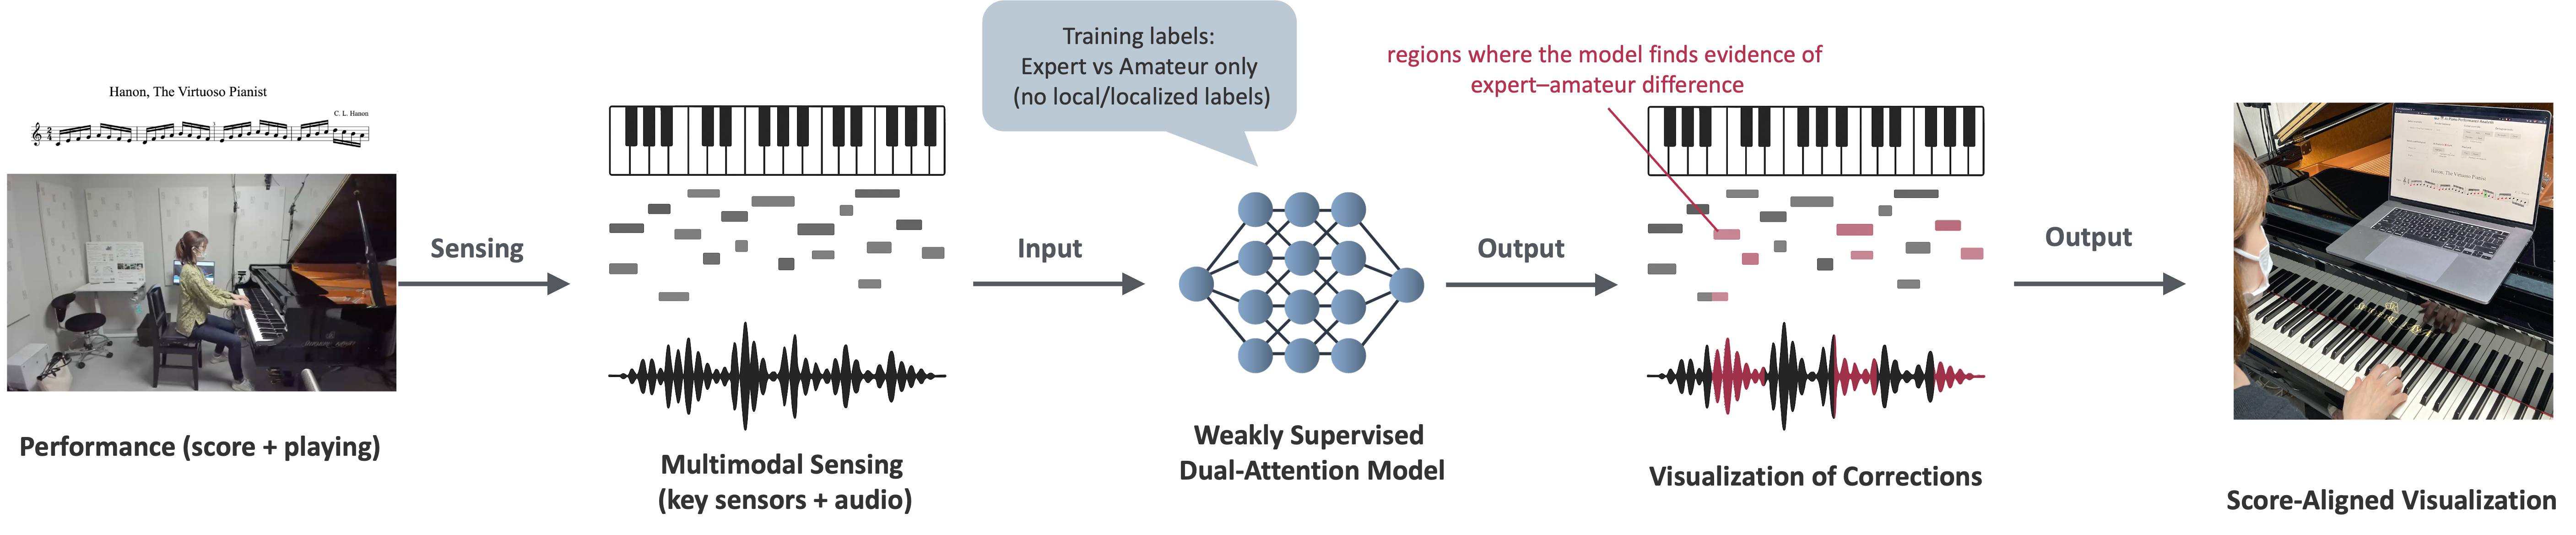
\includegraphics[width=\textwidth]{figures/teaser.png}
  \caption{\textbf{Profy: score-aligned highlights that focus practice.}From a single performance, our system produces red overlays on the score and waveform that show where a learner's playing diverges from expert renditions, helping pianists target passages for review instead of practicing everything uniformly. Under the hood, a weakly supervised dual-attention model---trained only with performance-level labels (Expert vs.\ Amateur), not per-note annotations---analyzes key-sensor (1\,kHz) and audio streams to localize these differences.}
  \Description{Left-to-right pipeline: Hanon score and a pianist photo; a panel labeled “Multimodal Sensing” with a keyboard schematic, piano-roll, and waveform; a “Weakly Supervised Dual-Attention Model” note stating “Training labels: Expert vs Amateur only (no localized labels)”; an “Output” panel where notes and waveform segments are shaded red to indicate stronger expert–amateur differences; and a final photo showing the score with red highlights. The figure communicates that coarse performance-level labels yield localized, score-aligned visualizations of where amateurs differ from experts.}
  \label{fig:teaser}
\end{teaserfigure}

%%
%% This command processes the author and affiliation and title
%% information and builds the first part of the formatted document.
\maketitle

% 日本語訳: 導入
% ======================================================================
% Section: Introduction
% ======================================================================
\section{Introduction}

Learning a creative skill like piano performance is not merely about avoiding wrong notes. It depends on subtle and context dependent nuances such as micro timing, articulation, and dynamic balance. Although teachers provide the contextual guidance that enables such growth, most practice occurs in isolation. As a result, feedback about nuance during lessons can be subjective and difficult to ground, and during solo practice formative feedback is largely absent. There is a need for methods that capture the subtle differences in nuance between expert and amateur performances and translate them into interpretable, localized feedback to guide practice and support teacher–student dialogue.

Existing educational tools and much prior research foreground accuracy metrics such as pitch, onset, and duration, which offers a narrow view of performance. Commercial platforms grade note correctness but provide little guidance on interpretive nuance, and surveys of automatic piano performance assessment report a persistent gap, since many systems output global scores rather than localized and actionable cues that teachers and learners can use~\cite{Kim2022APPA}. Many high performing models also remain opaque, and recent work on explainable AI for music stresses the need for musician centered explanations and interfaces that render model reasoning legible~\cite{BryanKinns2024}.

Our approach leverages sensing that has been underused in learning contexts. Modern digital pianos capture key motion at 1\,kHz, which preserves motor control signatures that audio alone can blur. We address the problem of localizing expertise dependent differences from coarse performance level labels and of presenting those differences as interpretable and score synchronized visualizations.

We present Profy, a weakly supervised system that discovers where a take departs from expert practice and renders those moments as score synchronized highlights. The model is trained only on performance level labels, namely expert or amateur, and produces time indexed evidence that can be overlaid on notation so that practice can focus on specific spans rather than on entire pieces.

We evaluate the approach on a multimodal corpus of short technical studies with synchronized key motion sensors and audio. The model distinguishes expert and amateur performances from these signals without using localized annotations. Analysis by piece shows that some items make the distinction clearer than others, which suggests practical choices when selecting material for practice or placement. An expert study with expert pianists indicates that the highlighted spans coincide with phrase boundaries, finger crossings, and dynamic changes that teachers routinely address.

The contributions of this paper are as follows.
\begin{enumerate}
\item We contribute a multimodal corpus of short technical studies for the analysis of expertise dependent differences, with synchronized 1\,kHz key sensors and audio collected from 80 participants over 2{,}433 sessions and 15 scale and arpeggio tasks.
\item We present a weakly supervised methodology that learns localized and interpretable evidence from performance level labels and produces score synchronized highlights that can guide practice.
\item We evaluate the system on our corpus, showing that multimodal signals reliably distinguish expert from amateur performances, localized highlights correspond to coachable passages, and certain pieces are particularly diagnostic for repertoire design.
\end{enumerate}







% ======================================================================
% Section: Related Work
% ======================================================================
\section{Related Work}

% 日本語訳: 本節では、我々のアプローチを動機づけ位置づける先行研究を三つの系譜に整理する。(§\ref{sec:rw-interactive})練習を足場づくりするインタラクティブ音楽学習システム、(§\ref{sec:rw-assessment})自動演奏評価とフィードバック、(§\ref{sec:rw-xai})音楽教育のための解釈可能AIである。いずれの領域でも、学習者と指導者が行動に移せる「局所的・解釈可能・楽譜同期」フィードバックの必要性を強調する。
We organize prior work into three strands that jointly motivate and situate our approach: (\S\ref{sec:rw-interactive}) interactive music learning systems that scaffold practice; (\S\ref{sec:rw-assessment}) automatic performance assessment and feedback; and (\S\ref{sec:rw-xai}) interpretable AI for music education. Across these areas, we emphasize the need for localized, interpretable, and score-synchronized feedback that learners and teachers can act on.

% ----------------------------------------------------------------------
% Subsection: Interactive Music Learning Systems
% ----------------------------------------------------------------------
\subsection{Interactive Music Learning Systems}
\label{sec:rw-interactive}

\subsubsection{Guidance on and around the keyboard.}
% 日本語訳: 初期研究の \emph{Piano Tutor} は初心者向けにリアルタイムの視覚フィードバックを提供した。投影型インタフェース(例: \emph{P.I.A.N.O.})は鍵盤上に手がかりを投影して練習を加速し、\emph{OnCall Piano Sensei} や \emph{piARno} のARオーバレイは運指や姿勢の案内を提示して音の正確さや手の位置を改善する。ウェアラブル/ハプティック設計もフィードバックを拡張し、\emph{MusicJacket} は弓使いの触覚キューを提示し、\emph{Mobile Music Touch} 手袋は受動的な触覚練習を支援する。これらのインタラクティブシステムは機械的正確さに有効で、学習初期の習得を促進する。
Early work such as Piano Tutor provided real-time visual feedback for amateur lessons~\cite{Dannenberg1992}. Projection-based interfaces (e.g., P.I.A.N.O.) accelerate practice by projecting cues onto the keyboard~\cite{Rogers2014}, and AR overlays in OnCall Piano Sensei and piARno present fingering and posture guidance that improves note accuracy and hand position~\cite{Chiang2015,Rigby2020}. Wearable and haptic designs further enrich feedback: MusicJacket delivers vibrotactile cues for bowing technique~\cite{Johnson2010}, and Mobile Music Touch gloves support passive haptic rehearsal\footnote{\url{https://www.freethink.com/series/superhuman/these-gloves-could-offer-rapid-recovery-from-brain-injuries}}. These interactive systems are effective for mechanical correctness and can boost early-stage learning~\cite{Yuksel2016}.

\subsubsection{Beyond note correctness.}
% 日本語訳: 一方で、多くのAR/VRピアノチュータは依然として音高・タイミングの正誤に重点を置き、テンポ一貫性・ダイナミクス・アーティキュレーションといった他の重要側面へのフィードバックを十分に提供していない。アクセシビリティや協調を志向する \emph{Piano Genie} や \emph{MirrorFugue} も、巧緻な技術分析より入口や共在感を優先する。注視計測で楽譜上の難所を特定・ハイライトする \emph{EyePiano} は、ターゲット化された練習への前進例である。
Despite their value, many AR/VR piano tutors still emphasize note-level guidance and ``fail to offer feedback on other essential aspects... such as tempo consistency, dynamics, and articulation''~\cite{Wilson2023VRPianoReview}. Accessibility- and collaboration-oriented interfaces like Piano Genie~\cite{Donahue2019} and MirrorFugue~\cite{xiao2011} similarly prioritize entry and co-presence rather than analysis of nuanced technique. A notable step toward targeted practice is EyePiano, which uses eye-tracking to identify and highlight difficult score passages~\cite{Karolus2023}.

% 日本語訳: 我々はこのデータ駆動の流れを継承しつつ、正誤から「熟達度に依存するニュアンス」へ焦点を移す。具体的には、1kHzの高解像度ピアノセンサ時系列から微細な運動技能の特徴を抽出し、練習を誘導する楽譜同期ハイライトとして提示する。これは主に音の正確さを扱ってきた既存のAR/ハプティック系を補完する。
We follow this data-driven trend while shifting focus from correctness to expertise-dependent nuance. Concretely, we leverage high-resolution piano sensor streams (1\,kHz) to reveal subtle motor-skill signatures and render them as score-aligned highlights that direct practice, complementing prior AR/haptic systems that mostly address note-level accuracy~\cite{Rogers2014,Chiang2015,Rigby2020,Johnson2010,Yuksel2016,Wilson2023VRPianoReview,Donahue2019,xiao2011,Karolus2023,Dannenberg1992}.

% ----------------------------------------------------------------------
% Subsection: Automatic Performance Assessment and Feedback
% ----------------------------------------------------------------------
\subsection{Automatic Performance Assessment and Feedback}
\label{sec:rw-assessment}

\subsubsection{From alignment to grading.}
% 日本語訳: 市販プラットフォーム(SmartMusic, Yousician など)は音高/タイミング誤りの検出に強いが、フィードバックを二値判断に還元しがちである。学術研究ではスコア–演奏整合と誤り検出が成熟し、DTWやHMMに基づくスコアフォローにより誤りや反復を含む演奏でも譜面に整合でき、エラーに頑健なリアルタイム伴奏などが可能になっている。整合を超えて、機械学習は全体熟達度の採点も行い、CNN/RNNで約80%精度、Transformer系(例: \emph{PianoBART})はシンボリック入力上でフレージングや表現を評価する。ただし、網羅的サーベイは、全体スコアや誤り数に留まり「局所的で行動可能」な指針が不足するギャップを指摘する。
Commercial platforms (e.g., SmartMusic, Yousician) robustly flag pitch and timing errors but largely reduce feedback to binary judgments. Academic work has matured score--performance alignment and error detection: dynamic time warping and HMM-based score following align performances to notation even with mistakes or repeats~\cite{nakamura2016}, enabling applications such as real-time accompaniment that tolerates errors and arbitrary repeats~\cite{nakamura2016}. Beyond alignment, ML models grade overall proficiency: CNN/RNN approaches report around 80\% accuracy, and transformer-based models (e.g., PianoBART) assess phrasing and expression on symbolic inputs~\cite{liang2024}. However, a comprehensive survey highlights a persistent gap: systems often produce global scores or error counts rather than localized, actionable guidance~\cite{Kim2022APPA}.

\subsubsection{Toward richer visual feedback.}
% 日本語訳: 研究プロトタイプは表現面の見える化の道筋を示す。\emph{Con Espressione} はテンポの微妙な揺れを可視化し、タイミングと音量のリアルタイム抽象可視化は学習者の表現再現能力を高める。テンポや強度の譜面注釈は演奏間比較を助け、アーティキュレーションやダイナミクスの自動評価もピアノ演奏の品質評価に有望である。一方で、多くは簡略化された素材や事前収録に制約され、学習者が表示から処方を推測する余地が大きい。
Research prototypes illustrate how expressive aspects can be made legible. Con Espressione visualizes timing deviations to expose tempo nuance~\cite{Widmer2017}. Real-time abstract visuals for timing and loudness improve learners’ ability to reproduce expressive detail~\cite{Sadakata2008}. Score annotations with tempo and intensity facilitate cross-performance comparison~\cite{Trevino2014}, and automatic evaluation of articulation and dynamics shows promise for quality assessment in piano playing~\cite{Phanichraksaphong2021}. Yet these systems are frequently constrained to simplified materials or predefined recordings and still leave learners to infer prescriptions from the displays.

% 日本語訳: 本研究はサーベイが指摘する「ラストマイル」に取り組む。すなわち、演奏が品質面で「どこで」乖離しているかを自動的に発見し、その情報を楽譜上に \emph{in situ} で提示して、具体的な練習ターゲットへと落とし込む。
In this space, we target the ``last mile'' identified by the survey~\cite{Kim2022APPA}: automatically discover where a take diverges in quality and present that information in situ on the score as concrete practice foci, while building on alignment and assessment advances~\cite{nakamura2016,liang2024,Widmer2017,Sadakata2008,Trevino2014,Phanichraksaphong2021,Kim2022APPA}.

% ----------------------------------------------------------------------
% Subsection: Interpretable AI for Music Education
% ----------------------------------------------------------------------
\subsection{Interpretable AI for Music Education}
\label{sec:rw-xai}

\subsubsection{Transparency and human–AI complementarity.}
% 日本語訳: 教室での採用は、AIのフィードバックが理解可能で人間の判断を補完するほど高まる。知的チュータリングでは、学習者の自己認識を支えるために意思決定過程の可視化が重視され、教室オーケストレーションでは教師は不透明なスコアより解釈可能な洞察を必要とする。創造領域では、AIは人間の専門性を上書きするのではなく拡張すべきとされる。
Adoption in classrooms increases when AI feedback is understandable and complements human judgment. Work in intelligent tutoring emphasizes making a system’s decision process visible to support learner self-awareness~\cite{Porayska2016}, and classroom orchestration tools find that teachers need interpretable insights rather than opaque scores~\cite{Holstein2019}. In creative domains, AI ought to augment, not override, human expertise\footnote{\url{https://ojs.aaai.org/aimagazine/index.php/aimagazine/article/view/7399}}.

\subsubsection{Musician-centered explanations and cross-domain cues.}
% 日本語訳: 音楽における説明可能AIの近年の議論は、演奏家中心の説明ツールの不足と、モデル出力を領域概念へ翻訳するインタフェースの必要性を指摘する。異領域デザインも示唆を与え、言語チュータでは波形上に発音の差異をハイライトする例がある。初心者ピアニストの研究でも、学習者は専門家が確実に検出する微妙な誤りを見落としがちで、その測定と可視化が有益であることが示される。
Recent work on explainable AI for music calls out the scarcity of musician-centered explanation tools and the need for interfaces that translate model outputs into domain concepts~\cite{BryanKinns2024}. Cross-domain designs show how aligned visualizations can surface subtle differences, as in a language tutor that highlights pronunciation divergences on a waveform display~\cite{Kawamura2021}. An amateur-pianist study similarly indicates that learners often overlook nuanced errors that experts reliably detect and benefit when such aspects are measured and visualized~\cite{Jiang2023}.

% 日本語訳: 以上を踏まえ、本研究は不透明な技能スコアを避け、解釈可能な「楽譜同期ヒートマップ」を採用する。弱教師ありのデュアルアテンションにより、教師の語彙と整合する人間可読の手がかりを生成し、チュータリング/教室の要請と整合させつつ演奏家中心のXAIを前進させる。
Responding to these threads, we eschew opaque skill scores in favor of an interpretable score-synchronized heatmap. A weakly supervised dual-attention model yields human-inspectable cues that align with teacher vocabulary, advancing musician-centered XAI while staying consistent with tutoring and classroom needs~\cite{Porayska2016,Holstein2019,BryanKinns2024,Kawamura2021,Jiang2023}.

% ----------------------------------------------------------------------
% NEW: Public corpora and sensing modalities
% ----------------------------------------------------------------------
\subsection{Public Piano Corpora and Sensing Modalities (Audio/MIDI vs.\ Motion)}
Widely used open corpora for piano focus on \emph{audio and/or MIDI} rather than high-rate key-motion sensing. \emph{MAESTRO} pairs aligned performance audio with MIDI from professional competitions and conservatories~\cite{Hawthorne2019MAESTRO}; \emph{MAPS} provides MIDI-aligned audio generated from MIDI or Disklavier recordings for transcription and alignment~\cite{Emiya2010MAPS}; and \emph{ASAP} offers precisely aligned scores and performances aimed at transcription research~\cite{Foscarin2020ASAP}. These resources have catalyzed AMT, alignment, and assessment research, but they do not include synchronized per-key motion at \(\geq 1\,\mathrm{kHz}\) across broad cohorts and standardized technique tasks (e.g., scales/arpeggios). This modality gap limits analyses of motor-skill micro-events (pre-touch latencies, key-travel profiles) that audio alone tends to smear.

% ----------------------------------------------------------------------
% NEW: High-resolution key-motion sensing in controlled studies
% ----------------------------------------------------------------------
\subsection{High-Resolution Key-Motion Sensing in Controlled Studies}
High-speed key-motion sensing has been leveraged in laboratory studies to probe motor control, often at millisecond resolution. Oku and Furuya built a non-contact deep-learning-based system achieving \(\sim1\,\mathrm{ms}\) temporal resolution on key motion~\cite{Oku2022Sensors}; Yasuhara \etal linked neural oscillations to fine motor timing during piano performance using synchronized EEG and key sensors~\cite{Yasuhara2024iScience}; and recent work argues for the \emph{motor origins of timbre} in piano performance, supported by high-resolution key-motion measurements~\cite{Kuromiya2025PNAS}. To our knowledge, however, such sensing has not materialized as a \emph{public, multi-participant corpus} with standardized technique tasks, consistent capture protocol, and documentation suitable for benchmarking.

% ----------------------------------------------------------------------
% NEW: Positioning our resource contribution
% ----------------------------------------------------------------------
\subsection{Positioning of This Corpus Contribution}
The approach in this paper addresses the above gap by documenting a corpus of short technical studies with synchronized 1\,kHz per-key motion and 44.1\,kHz audio, adjudicated performance-level labels, and a data-card style schema. Whereas audio/MIDI corpora (\S\ref{sec:rw-assessment}) support alignment and global assessment, the present resource is designed for \emph{expertise-dependent motor-skill analysis} and for \emph{interpretable, score-synchronized feedback}. We therefore complement prior datasets by adding a sensing modality that is essential for localizing practice-relevant micro-events, while remaining compatible with score-based UI overlays grounded in established alignment methods~\cite{nakamura2016}.






% ----------------------------------------------------------------------
% Section: Dataset: Corpus and Task Suite
% ----------------------------------------------------------------------
\section{Dataset: Corpus and Task Suite}
\label{sec:dataset}

Compared with widely used audio/MIDI datasets~\cite{Hawthorne2019MAESTRO,Emiya2010MAPS,Foscarin2020ASAP} and surveys of automatic piano performance assessment (APPA)~\cite{Kim2022APPA}, publicly available resources seldom include synchronized \emph{high‑rate} per‑key motion (~$\approx$1\,kHz) for \emph{short technical studies}. Our corpus is designed to address this practical gap by pairing 88‑key motion at 1\,kHz with 44.1\,kHz audio under a standardized protocol, enabling localized and interpretable analyses of expertise‑dependent motor skills. Detailed comparisons to prior corpora are provided in §Related~Work; here we document the resource for reproducible use.

\begin{table*}[t]
  \centering
  \caption{\textbf{Corpus at a glance. All values computed from the data directory.}}
  \label{tab:profy_glance}
  \begin{tabular}{@{}ll@{}}
    \toprule
    Item & Value \\
    \midrule
    Participants (unique) & 80 \\
    Sessions (total / adopted) & 2{,}433 / 1{,}175 (48.3\%) \\
    Piece tasks (unique) & 15 (9 scales, 6 arpeggios) \\
    Takes per piece (mean / median / max) & 2.17 / 2 / 10 \\
    Take length (median [min, max]) & 10.53\,s [1.37, 246.75] \\
    Modalities & 1\,kHz per‑key motion; 44.1\,kHz stereo audio; optional multi‑view video, posture, pedal \\
    Labels & \texttt{Expert} / \texttt{Amateur} (performance‑level) \\
    \bottomrule
  \end{tabular}
\end{table*}

\subsection{Scope and Novelty}
\label{subsec:scope}
The contribution is a corpus expressly targeted at expertise‑dependent motor‑skill analysis on short, controlled materials, with synchronized high‑rate sensing. Each take contains 88‑channel key‑motion at 1\,kHz and stereo audio at 44.1\,kHz, captured under a consistent protocol. As far as we are aware, public resources commonly used for performance analysis focus on audio and/or MIDI and do not offer high‑rate per‑key motion suitable for localizing micro‑events associated with technique~\cite{Hawthorne2019MAESTRO,Emiya2010MAPS,Foscarin2020ASAP}. Surveys of APPA likewise note that corpora for interpretable, localized feedback are scarce and typically omit sensor streams beyond audio~\cite{Kim2022APPA}. To our knowledge, there is no publicly accessible corpus of short technical studies (scales/arpeggios) with synchronized 1\,kHz key‑motion and 44.1\,kHz audio comparable in scope to ours.

\subsection{Protocol and Task Suite}
\label{subsec:protocol}
We recruited eighty pianists spanning a broad proficiency range from amateurs to experienced performers and teachers. Eligibility required the ability to play major and minor scales and triad arpeggios hands together at a comfortable tempo; recent injury and hearing conditions were exclusionary. Personally identifying information was not stored with the recordings.

Performances were captured on a digital piano instrumented for per‑key motion at 1\,kHz across all eighty‑eight keys. Audio was recorded at 44.1\,kHz and 32‑bit float with fixed microphone placement in a quiet room. The sensor and audio streams were hardware‑synchronized to a common timestamp epoch, ensuring sample‑accurate alignment suitable for cross‑modal analysis and later score following~\cite{nakamura2016}.

The task suite consists of fifteen short studies selected to isolate core motor demands while minimizing confounds from long‑form repertoire. Nine tasks are scales and six are arpeggios. The scale tasks use key signatures that create contrasting patterns of white and black keys: B, C, Des, Es, and Ges major together with b, cis, es, and fis minor. A scale here means a stepwise traversal of the notes defined by a key signature over one or more octaves, ascending and descending in a fixed pattern. For non‑specialists, the salient technical challenge in scales is maintaining evenness of timing and loudness while executing \emph{finger crossings}—a coordinated “thumb‑under/finger‑over” maneuver that allows the hand to reposition without audible bumps. Keys dominated by black keys alter hand posture and finger travel: C major largely uses white keys and demands economy in frequent crossings, whereas Ges major uses many black keys and changes the angle and surface contact of the fingers, which affects control of attack and release. Minor keys introduce raised leading tones in harmonic or melodic forms, subtly changing fingerings and local difficulty around scale degrees 6–7.

The arpeggio tasks use As, D, and F major together with b, f, and gis minor. An arpeggio is a chord played as a sequence of its tones rather than simultaneously, typically across multiple positions or octaves. Technically, arpeggios stress controlled hand relocation and span management. The player must rotate and translate the wrist to place the hand over successive chord tones, coordinate forearm movement to bridge larger gaps, and regulate pedal so that changes of position do not smear. Compared with scales, arpeggios create asymmetric motion between hands, more varied inter‑onset intervals, and larger vertical displacements on the keyboard, all of which challenge consistency of tone and timing. These differences yield complementary motor signatures in the key‑motion data and provide a richer testbed for distinguishing expertise.

Session flow was simple and uniform. After brief instructions and an optional warmup, each participant could record multiple takes per task with a cap of ten; across the dataset the median is two takes and the mean is 2.17. Tempo was self‑selected unless otherwise indicated. Participants were asked to aim for steady timing and even dynamics rather than concert speed, emphasizing technique over display. To reduce order effects, task order was randomized across sessions.

The piece names in the metadata follow German pitch notation, where Des, Es, and Ges correspond to D$\flat$, E$\flat$, and G$\flat$; As denotes A$\flat$; cis, fis, and gis correspond to C$\sharp$, F$\sharp$, and G$\sharp$; and the single letter b denotes B$\flat$. Where “dur” and “moll” appear, they indicate major and minor, respectively. We keep these names as recorded to preserve reproducibility.

\subsection{Labels, Curation, Contents, Uses, and Limitations}
\label{subsec:labels-content}
Each take carries a performance‑level label, \texttt{Expert} or \texttt{Amateur}, derived from human ratings. Fifty‑three raters provided 6{,}517 ratings over 1{,}083 unique takes, with a median of four ratings and a mean of 6.01 ratings per take. The recorded rater‑side tags map directly to the two labels (\texttt{pro}→\texttt{Expert}, \texttt{amateur}→\texttt{Amateur}), yielding 597 expert‑labeled and 486 amateur‑labeled takes among the rated subset. No localized annotations were used for model training; the piece‑wise analyses in §\ref{sec:technical-eval} rely only on these global labels.

Curation was conservative. A session was adopted only if the capture was intact, the protocol was followed, and the content was valid for the declared task. Of 2{,}433 sessions, 1{,}175 (48.3\%) were retained, which is reflected by an \texttt{isAdopted} flag in the accompanying CSV. For each take we compute basic indicators of acoustic reliability—non‑silence ratio, spectral flatness, and loudness—which are included as metadata so that users can filter analyses by estimated quality or replicate our ablations.

The released structure is straightforward. Each adopted session contains synchronized key‑motion streams at 1\,kHz for all eighty‑eight keys and stereo audio at 44.1\,kHz, alongside per‑take metadata that records identifiers, the task key, and the quality indicators noted above. For many takes we also provide derived per‑note information such as onset and offset times and basic kinematic summaries; additional modalities, including multi‑view video, posture or skeleton traces, and pedal signals, are available for a subset. Key‑motion values are normalized displacements in arbitrary units centered near zero. All time bases are in seconds, and the frame rates are explicitly recorded with each take.

The corpus supports three benchmark families that we use in §\ref{sec:technical-eval}: expert‑versus‑amateur classification from sensors, from audio, or from both; weakly supervised localization of amateur weaknesses using performance‑level labels; and analysis of diagnosability at the piece level. When a score transcript and reliable score following are available~\cite{nakamura2016}, evidence learned from weak supervision can be aggregated to notes or beats and rendered on the staff; otherwise, we use timeline overlays that align by absolute time.

The scope is intentionally focused, which brings both strengths and limitations. Short, controlled studies and a consistent capture setup make it feasible to detect sub‑second motor events that are often blurred in audio alone and to compare takes fairly across players. At the same time, ecological validity is narrower than in long‑form repertoire recorded across diverse environments, and some optional modalities are incomplete across sessions. Access, licensing, and release logistics are omitted here due to anonymized review. Within those bounds, the corpus foregrounds synchronized, high‑rate sensing for interpretable feedback research and, to our knowledge, fills a gap left by audio/MIDI‑centric corpora~\cite{Hawthorne2019MAESTRO,Emiya2010MAPS,Foscarin2020ASAP} and resources catalogued in APPA surveys~\cite{Kim2022APPA}.





\begin{figure*}[t]
  \centering
  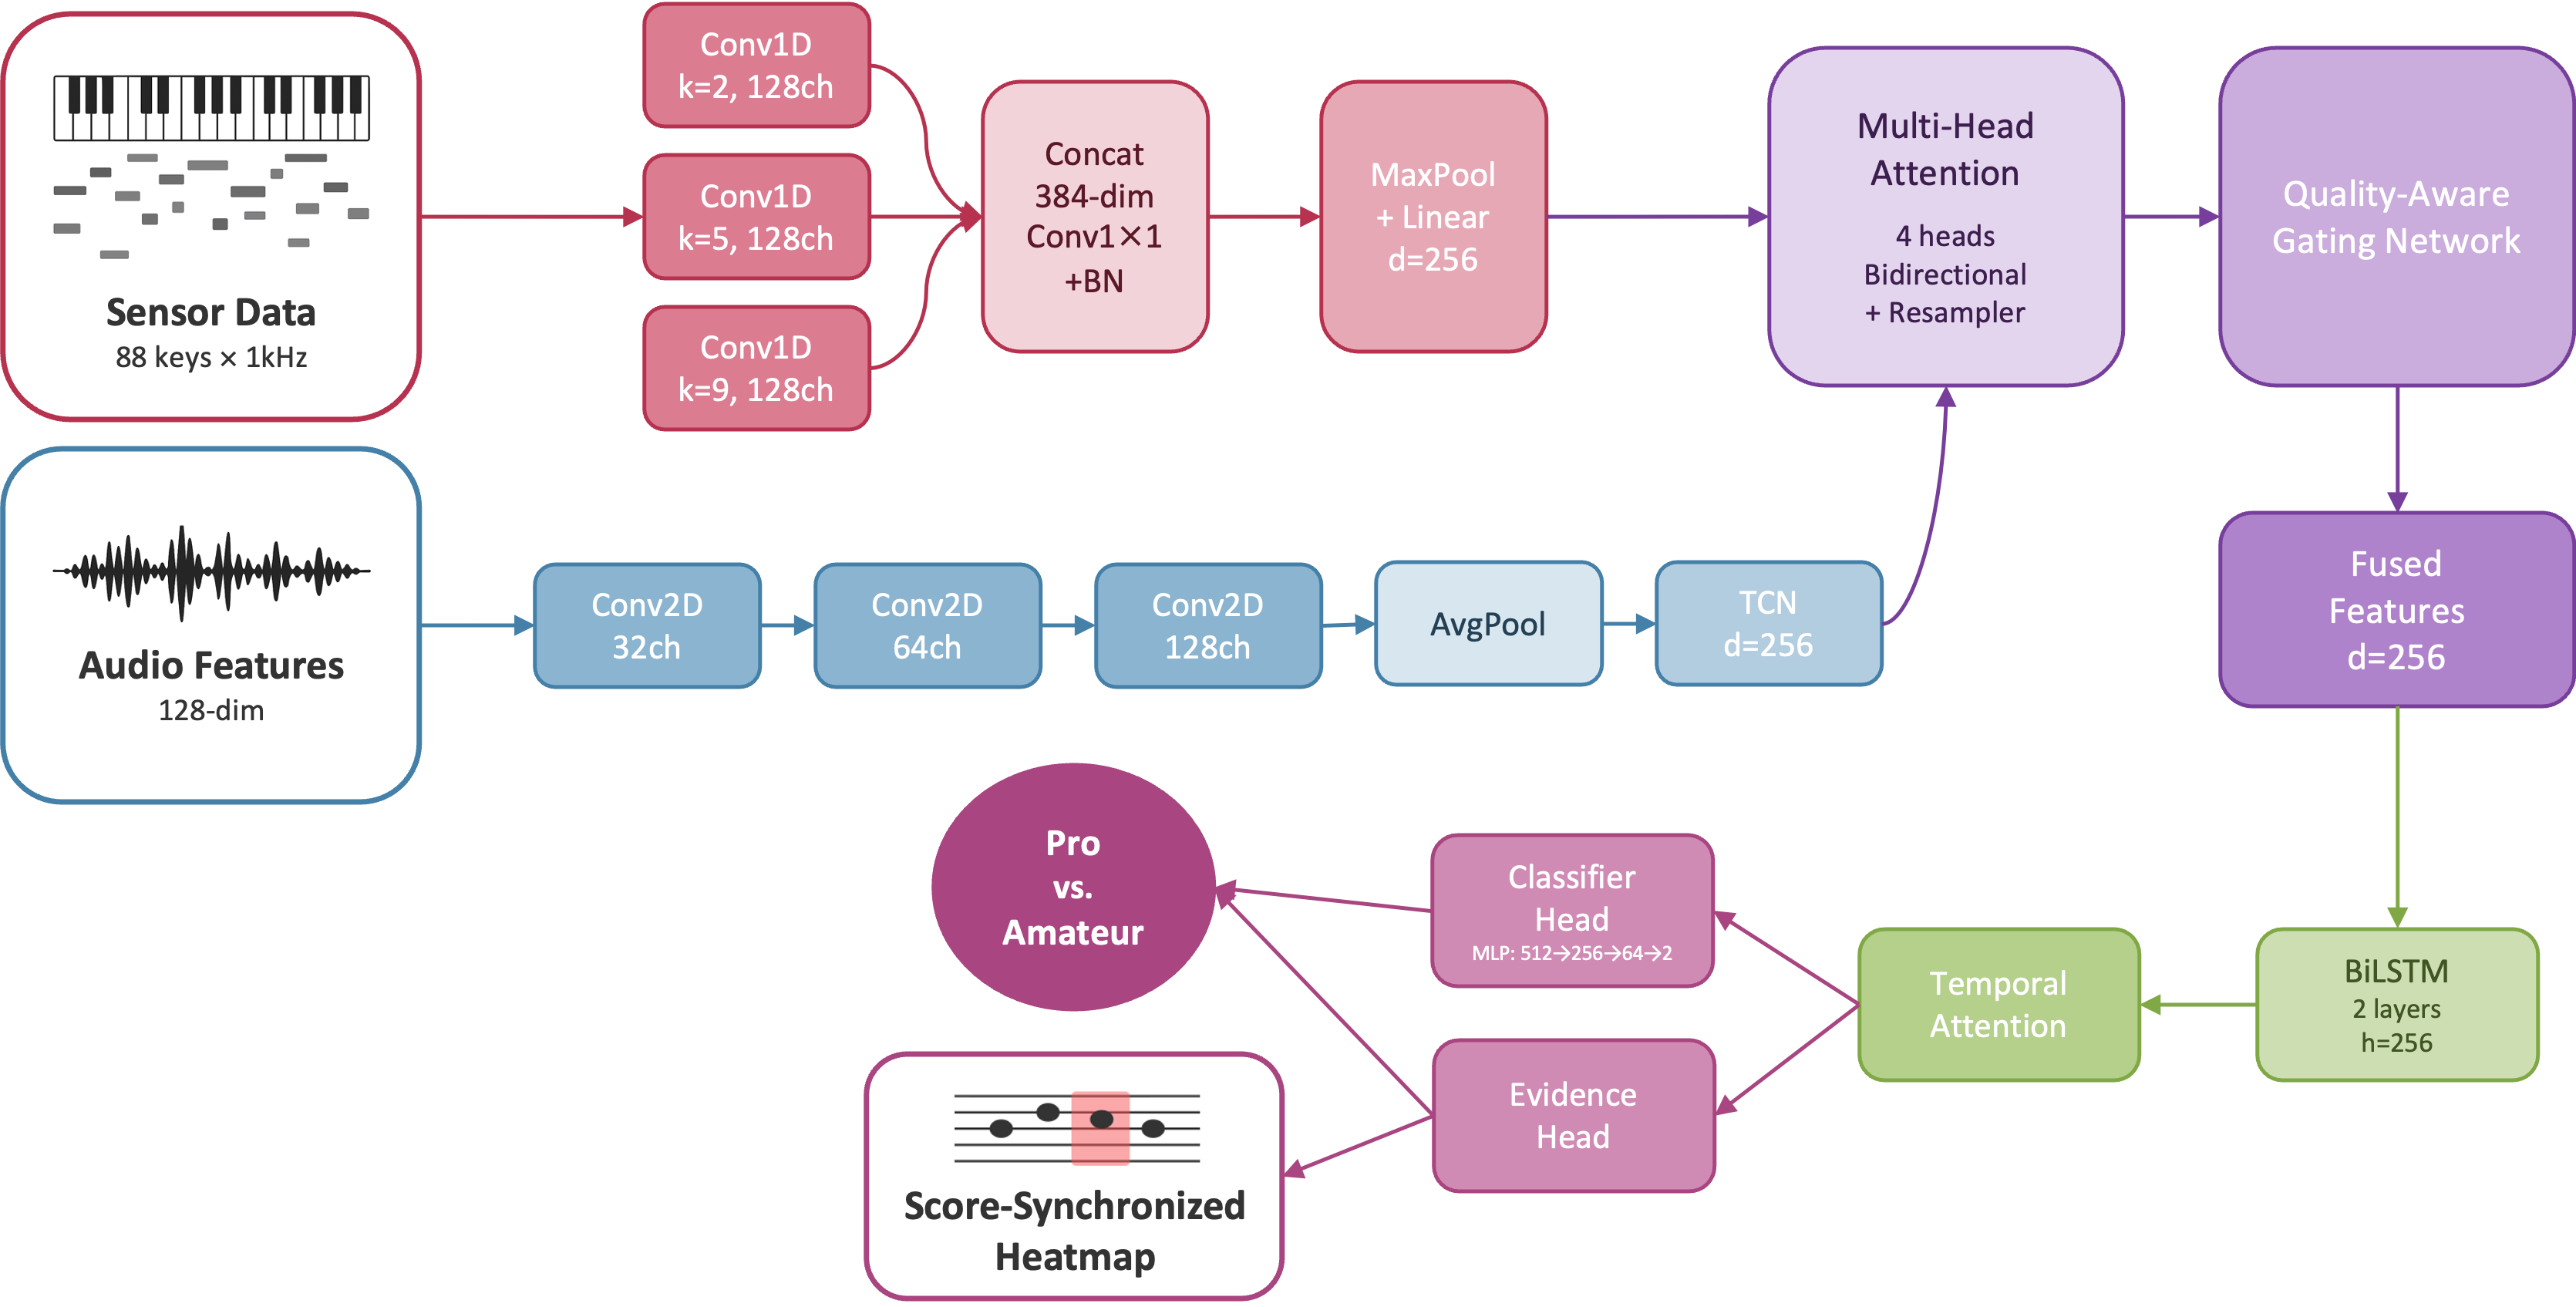
\includegraphics[width=0.9\linewidth]{figures/architecture_overview.png}
  \caption{\textbf{Profy architecture.} Two modality-specific encoders transform (top) 88-key, 1\,kHz sensor streams and (bottom) 128‑dim audio features into $d{=}256$ sequences. A 4‑head bidirectional multi‑head attention block with a learnable resampler exchanges information across modalities~\cite{Vaswani2017,Lu2019ViLBERT}. A quality‑aware gating network, conditioned on acoustic quality indicators (NSR, spectral flatness, loudness), mixes four candidates into a fused representation. A 2‑layer BiLSTM with temporal attention produces per‑frame evidence and an attention‑pooled clip representation for expert/amateur classification; an auxiliary MIL objective guides evidence localization~\cite{Ilse2018,Pinheiro2015}.}
  \Description{Architecture diagram of the Profy model showing six stages: input processing, dual encoding, cross-modal attention, quality-aware fusion, temporal aggregation, and dual-head output with visualization.}
  \label{fig:architecture_overview}
\end{figure*}




% ======================================================================
% Section: Profy: Methodology and Architecture
% ======================================================================
\section{Profy: Methodology and Architecture}

\subsection{System Overview}
\label{subsec:overview}
Profy processes two synchronized streams per performance and converts them into interpretable guidance. The system ingests an 88–channel key-motion sensor time series $\mathbf{S}\in\mathbb{R}^{T\times 88}$, uniformly resampled from 1\,kHz to a fixed $T$ frames, together with a stacked audio feature map $\mathbf{A}\in\mathbb{R}^{T\times 128}$ computed from 22.05\,kHz mono audio. An audio quality vector $\mathbf{q}=[\mathrm{NSR},\mathrm{SFlat},\mathrm{Loud}]$ and a non-silence mask $\mathbf{m}$ accompany the audio stream. Modality-specific encoders transform the inputs; bidirectional cross-modal attention aligns and exchanges information~\cite{Vaswani2017,Lu2019ViLBERT}; and a quality-aware gate fuses four candidate sequences into a single representation. A BiLSTM with two heads then produces per-frame evidence and a clip-level classification from an attention-pooled context. The UI receives a global expert probability, a time-localized evidence curve, a timeline severity profile used to draw overlays, and reliability flags that suppress overlays when inputs are untrustworthy. Figure~\ref{fig:architecture_overview} provides a graphical summary of this pipeline. For localization without frame labels we use an auxiliary MIL objective~\cite{Pinheiro2015,Ilse2018}.

\subsection{Inputs and Outputs}
\label{subsec:io}
The task is to predict a binary expertise label $y\in\{0,1\}$ (expert/amateur) for an entire performance while learning time-localized signals from performance-level labels only. The input consists of a sensor stream $\mathbf{S}\in\mathbb{R}^{T\times 88}$ (per-key positions resampled/padded to length $T$), an audio feature stream $\mathbf{A}\in\mathbb{R}^{T\times 128}$ comprising Mel, MFCC, reduced chroma, tonnetz, spectral contrast, and frame statistics, and two auxiliary quantities---a non-silence mask $\mathbf{m}\in\{0,1\}^T$ and the quality vector $\mathbf{q}\in\mathbb{R}^{3}$. When available, a frame-to-score mapping $\phi:t\mapsto n$ from score following can be used at rendering time; by default the UI draws timeline overlays. The system returns four outputs that the UI consumes directly: a global expert probability $\hat{y}\in(0,1)$, a per-frame evidence sequence $e_{1:T}\in[0,1]^T$ that localizes decisive moments, a timeline severity profile $s_{1:T}$ used to control overlay opacity, and a compact set of reliability flags indicating low audio SNR, uncertain alignment, insufficient clip length, or missing sensor channels.

\begin{table}[t]
  \centering
  \caption{Notation used in the method.}
  \label{tab:notation}
  \begin{tabular}{@{}ll@{}}
    \toprule
    Symbol & Meaning \\
    \midrule
    $T$ & Frames per take (default $T{=}1000$) \\
    $\mathbf{S}\in\mathbb{R}^{T\times 88}$ & Sensor time series (key position) \\
    $\mathbf{A}\in\mathbb{R}^{T\times 128}$ & Audio feature time series \\
    $\mathbf{m}\in\{0,1\}^{T}$ & Non-silence mask (audio) \\
    $\mathbf{q}=[\mathrm{NSR},\mathrm{SFlat},\mathrm{Loud}]$ & Audio quality vector \\
    $e_t\in[0,1]$ & Per-frame evidence (visualization) \\
    $\alpha_t\in(0,1)$ & Attention weight ($\sum_t \alpha_t{=}1$) \\
    $\hat{y}\in(0,1)$ & Global expert probability (clip-level) \\
    $s_t$ & Severity (timeline) \\
    \bottomrule
  \end{tabular}
\end{table}

\subsection{Preprocessing and Leakage Controls}
\label{subsec:preproc}
All sequences are uniformly resampled (or zero-padded) to a fixed temporal length $T{=}1000$ without sliding windows so that each take produces one example. For sensors, we read the 88 key channels and resample/pad to $T$; no additional per-fold normalization is applied. Audio is downmixed to mono at 22.05\,kHz and converted into an 80-dimensional Mel filterbank, 20 MFCCs, 9 chroma coefficients (obtained by variance-based reduction from 12), 6 tonnetz features, 5 spectral-contrast values with $n_{\text{bands}}{=}4$, and eight frame-level statistics (spectral centroid, bandwidth, rolloff, flatness, spectral flux, ZCR, RMS, and $\Delta$RMS), stacked to 128 dims using standard implementations in \texttt{librosa}~\cite{mcfee2015librosa}, with tonnetz and spectral-contrast following~\cite{HarteSandler2006,Jiang2002}. The non-silence mask $m_t$ uses short-term RMS with a hop chosen to yield $T$ frames:
\[
m_t=\mathbb{1}\![\mathrm{RMS}_t>0.3\,\overline{\mathrm{RMS}}],\qquad
\mathrm{NSR}=\frac{1}{T}\sum_{t=1}^T \mathbb{1}\![\mathrm{RMS}_t>0.5\,\overline{\mathrm{RMS}}].
\]
Spectral flatness and loudness (dB) are averaged over $\{t\mid m_t{=}1\}$. To avoid any train–test leakage, audio features are standardized \emph{per fold} using statistics computed on the \emph{training split only} (non‑silent frames). The per-fold mean and standard deviation are persisted and applied to the corresponding validation/test data within that fold.

\subsection{Model Architecture}
\label{subsec:arch}
\subsubsection{Encoders}
The sensor encoder applies three temporal one-dimensional convolutions with kernel sizes $3$, $5$, and $9$ and 128 channels each to $[B,T,88]$; the three outputs are concatenated, compressed by a $1{\times}1$ convolution followed by batch normalization, ReLU, and max pooling with stride $2$, and then projected to a hidden dimensionality $d{=}256$. The audio encoder treats $[B,T,128]$ as a spectro-temporal map $[B,1,128,T]$, processes it with a 2D CNN of widths $1\!\to\!32\!\to\!64\!\to\!128$, averages over the frequency axis, linearly projects to $d$, and finishes with two temporal convolutional blocks of dilations $1$ and $2$~\cite{Bai2018TCN}. A downsampled version of the non-silence mask gates the activations so that silent regions do not dominate the representation.

\subsubsection{Cross-modal Attention}
Bidirectional cross-attention allows either modality to query the other and resolve ambiguities between motor control and acoustic outcome. We use four attention heads in each direction and a learnable resampler to reconcile small residual length mismatches. The result is a pair of length-$T$ sequences in the shared hidden space whose elements have been exposed to the complementary stream~\cite{Vaswani2017,Lu2019ViLBERT}.

\subsubsection{Quality-aware Gating (D2)}
\label{subsec:gating}
After cross-attention, the model forms four candidate sequences: the plain sensor encoding, the audio-to-sensor attended sequence, the resampled audio encoding, and the sensor-to-audio attended sequence. Time-averaged summaries of the sensor and audio streams are concatenated with a projection of the quality vector $\mathbf{q}$ and passed through a small MLP that outputs four raw mixture logits. A temperature softmax converts logits to weights with temperature $1+\gamma(1{-}\mathrm{NSR})$ (with $\gamma{=}2.0$). The combined sensor share (plain+attended) is then floored adaptively based on NSR within $[0.35,0.6]$ before renormalization, preventing noisy audio from overwhelming cleaner sensor evidence. This gating behaves as a mixture-of-experts controller~\cite{Jacobs1991MoE,Shazeer2017MoE}.

\subsubsection{Temporal Modeling and Dual Heads}
A two-layer BiLSTM with hidden size $256$ and dropout $0.2$ models temporal context over the fused sequence and feeds two parallel heads. The evidence head produces per-frame scores $e_t\in[0,1]$ used for visualization and auxiliary MIL training. The classifier head pools the BiLSTM outputs with learned temporal attention $\alpha_t$ and maps the pooled context to a clip-level expert/amateur decision. The total number of trainable parameters is approximately $4.16\,\mathrm{M}$ for the final architecture. Latency is reported under a consistent condition ($T{=}1000$, batch size $1$): about $\sim$38\,ms on an RTX\,3090 (p95 52\,ms), $\sim$78\,ms on an RTX\,2060 (p95 105\,ms), and $\sim$260\,ms on an i7‑1185G7 CPU (p95 360\,ms), supporting in-the-loop feedback.


\subsection{Weak Supervision and Objective}
\label{subsec:weak}
The final objective uses only the regularization terms actually employed in the released code. The primary loss is cross-entropy on the clip-level logits. To encourage faithful localization without frame labels, we add two auxiliary terms on the evidence $e_t$: (i) a multiple‑instance learning (MIL) objective that treats $1-\prod_t(1{-}e_t)$ as the clip‑level positive probability and applies BCE to the expert label (weight $\lambda_{\mathrm{mil}}{=}0.5$), and (ii) an $\ell_1$ sparsity term on $e_t$ (weight $\lambda_{\mathrm{evi}}{=}0.001$). For multimodal training, we regularize the modality gate by encouraging diverse (high‑entropy) mixtures via an entropy term on the modality weights (weight $\lambda_{\mathrm{ent}}{=}0.1$). We \emph{do not} use total‑variation on $e_t$, KL alignment, or log‑sum‑exp pooling in the final experiments.

\subsection{From Inference to UI: Evidence$\rightarrow$Overlays}
\label{subsec:viz}
We compute a timeline severity as the product of attention and evidence, optionally smoothed and normalized for display. In our overlay tool, severity is scaled by a small power (e.g., $\rho\approx1.5$) and a short moving-average window (e.g., 9) to improve readability. By default, overlays are drawn on a timeline; when a score transcript and successful score following are available~\cite{nakamura2016}, the same severity can be aggregated to notes or beats and rendered on the staff.

\subsection{Design Decisions (D1–D6) and Alternatives}
\label{subsec:design}
The choice of weak supervision (D1) rests on the practical constraint that only performance-level labels are available; we supervise the clip decision directly and use MIL on evidence as an auxiliary to encourage localized cues. The quality-aware gating (D2) incorporates audio reliability via NSR-dependent temperature and an adaptive sensor-share floor. Decoupling evidence and decision heads (D3) proved important: a single head with post-hoc saliency produced less stable highlights. Separating mid-level gated fusion—which drives evidence—from decision-level fusion used for headline metrics (D4) prevents small accuracy gains from compromising readability. Normalizing time to $T{=}1000$ (D5) keeps model capacity in check; overlays are drawn on a timeline by default, with optional mapping to score when transcripts are available. Finally, the system is designed to fail gracefully (D6): when inputs are unreliable, it suppresses overlays and explains why, rather than drawing potentially misleading highlights.

\subsection{Splits and Reproducibility}
All results are produced with a three‑fold \texttt{GroupKFold} using a \emph{single} group vector at the \emph{performer} level (the same performer never appears across folds). Within each training split, fifteen percent of the data is reserved for validation. Random seeds are fixed at $42$ for PyTorch, NumPy, and data‑loader workers, and deterministic flags are set where available. Audio parameters include a sampling rate of 22.05\,kHz, FFT size $n_{\text{fft}}{=}2048$, a hop chosen to yield $T$ frames, 80 Mel bands, 20 MFCCs, 6 tonnetz dimensions, four spectral‑contrast bands, and nine chroma dimensions after reduction. No positional encodings are used; temporal structure is modeled entirely by the BiLSTM. Configuration files in YAML format specify data paths, feature extraction, architecture, and training hyperparameters; code, configs, and a deterministic inference script are archived with commit hashes and an exported environment file so that results can be reproduced exactly. For reproducibility, we fix the software stack to Python~3.10, PyTorch~2.3, CUDA~12.1, cuDNN~8.9, librosa~0.10, and numpy~1.26 (versions indicative). Grouped cross‑validation uses \texttt{GroupKFold} from scikit‑learn~\cite{Pedregosa2011Scikit}. Optimization employs AdamW~\cite{LoshchilovHutter2019AdamW}. In supplementary experiments, we also report held‑out piece evaluations (LOPO/LOK) to assess generalization to unseen keys/pieces.





% 日本語訳: 拡張技術評価
% ======================================================================
% Section: Technical Evaluation
% ======================================================================
\section{Technical Evaluation}\label{sec:technical-eval}

% 日本語訳: 冒頭で図2の全体アーキテクチャに触れ、本節での評価の文脈を示す。
As overviewed in Figure~\ref{fig:architecture_overview}, Profy processes sensor and audio streams with dual encoders, couples them via bidirectional cross-modal attention, and fuses features with a quality-aware gate before temporal modeling and dual heads (evidence and classifier). This architecture yields both a global decision (expert/amateur) and time-localised evidence curves that underpin our visualisations.

\noindent\textit{What is new compared to prior work.}
Without overselling, our approach differs in three practical ways relevant to evaluation:
\begin{itemize}
  \item \textbf{Weak-supervision with localized signals}: Trained only on performance-level labels, the model still produces time-indexed evidence usable for score-synchronised highlights; many prior APPA systems report global scores without localized cues. Our visual outputs are qualitatively cross-checked with expert judgment (\S\ref{sec:technical-eval}).
  \item \textbf{Multimodal, quality-aware fusion}: We combine high-resolution key-sensor data with audio, using bidirectional cross-modal attention and a gate informed by acoustic quality (e.g., NSR, spectral flatness, loudness) to stabilise fusion.
  \item \textbf{Separation of accuracy and interpretability paths}: Reported metrics use decision-level fusion for robustness, while mid-level attention/evidence is preserved for UI-facing explanations—preventing one objective from compromising the other.
\end{itemize}
\noindent\textbf{Results at a glance.}
Within this section, we provide results that correspond to the above points: (R1) On \emph{expert vs. amateur} classification, sensor-only and multimodal models achieve Macro-F1 $\sim$0.69 and $\sim$0.67 respectively (Table~\ref{tab:main_results}). (R2) By \emph{modality and piece}, sensor-only exceeds audio-only and scales tend to be easier than arpeggios (piece-wise analysis and figures in \S\ref{sec:technical-eval}). (R3) For \emph{localized highlights}, qualitative cross-checks against expert-marked segments and correlations with dataset proxies support that severity hotspots coincide with pedagogically salient weaknesses (\S\,Highlight Validity).
We now evaluate these outputs quantitatively using 3-fold cross-validated results, reporting only model-generated metrics and visualisations.


% 日本語訳: ・Cross Validation and Generalization
% ----------------------------------------------------------------------
% Subsection: Cross-Validation and Generalization
% ----------------------------------------------------------------------
\subsection{Evaluation Goals and Protocol}

\textbf{Goals.}
We evaluate three core questions: (G1) Can the model reliably classify \emph{expert vs. amateur} performances under group splits? (G2) Which \emph{inputs and pieces/keys} are easier or harder to separate (via modality ablations and piece-wise analysis)? (G3) Do the \emph{highlights} localise \emph{amateur weaknesses} in a way that is pedagogically meaningful (expert cross-check and data proxies)?

\textbf{Protocol.}
We use 3-fold GroupKFold grouped \emph{by performer} to prevent leakage across subjects. Metrics are Macro-F1 and accuracy averaged over folds. Reported metrics use decision-level fusion; mid-level attention/evidence is retained for visualisation but not used in the loss.

\textbf{Main results.}
Table~\ref{tab:main_results} summarises the cross-validated results. Sensor-only achieves Macro-F1 $0.687\,\pm\,0.092$ (accuracy $0.708\,\pm\,0.070$), audio-only reaches Macro-F1 $0.603\,\pm\,0.022$ (accuracy $0.611\,\pm\,0.019$), and multimodal fusion attains Macro-F1 $0.672\,\pm\,0.075$ (accuracy $0.698\,\pm\,0.043$). Fold-level Macro-F1 ranges are: sensor $0.583$--$0.807$, audio $0.574$--$0.629$, multimodal $0.567$--$0.733$.

% 日本語訳: 特徴の重要性と解釈性
% ----------------------------------------------------------------------
% Subsection: Feature Importance and Interpretability
% ----------------------------------------------------------------------
\subsection{Feature Importance and Interpretability}

% 日本語訳: 特性貢献分析
\textbf{Feature Contribution Analysis.}
% 日本語訳: 本稿ではモダリティ単体と融合の性能から寄与を概観する。
We characterise modality contributions via modality-specific and fused models. As summarised in Table~\ref{tab:main_results}, the sensor stream performs strongest on its own, the audio stream trails slightly, and decision-level fusion approaches the sensor baseline while improving over audio-only across folds.

% (Removed modality bar figure per reviewer preference; table suffices.)

% 日本語訳: 注意解釈
\textbf{Attention Interpretability.}
% 日本語訳: 本節では図示を行わず、定量評価の結果のみを提示する。
We focus this section on quantitative metrics; visual case studies are omitted here.

\begin{table}[t]
  \centering
\caption{Cross-validated performance on expert vs. amateur classification (3-fold GroupKFold). Values are mean $\pm$ SD over folds.}
  \label{tab:main_results}
  \begin{tabular}{lcc}
    \hline
    Mode & Macro-F1 & Accuracy \\
    \hline
    Sensor-only & 0.687 $\pm$ 0.092 & 0.708 $\pm$ 0.070 \\
    Audio-only  & 0.603 $\pm$ 0.022 & 0.611 $\pm$ 0.019 \\
    Multimodal  & 0.672 $\pm$ 0.075 & 0.698 $\pm$ 0.043 \\
    \hline
  \end{tabular}
\end{table}

% 日本語訳: エラー分析と失敗モード
\subsection{Error Analysis and Failure Modes}

% 日本語訳: 混乱分析
\textbf{Confusion Analysis.}
Across all held‑out folds (6{,}476 test items; total test support aggregated over 3 folds), the multimodal model misclassifies 1{,}957 performances (30.2\%). Aggregated over folds, class‑wise recall is $0.537$ for class~0 (amateur) and $0.813$ for class~1 (expert), consistent with the Macro‑F1 in Table~\ref{tab:main_results}.

\subsection{Piece-wise Accuracy and Piece Set}
\textbf{Why piece-wise analysis.}
Scales and arpeggios impose different motor demands (evenness, crossing, stretch), and keys differ in black/white-key patterns. We therefore analyse accuracy by \emph{piece} to reveal technique-specific strengths and weaknesses.

\textbf{Piece set overview.}
The evaluation covers 15 study pieces: 9 \emph{scales} (B, C, Des, Es, Ges majors; b, cis, es, fis minors) and 6 \emph{arpeggios} (As, D, F majors; b, f, gis minors). Aggregated over folds, this yields 6{,}476 test predictions (total support), with piece-averaged accuracy $0.696$. By category, scales achieve mean piece-averaged accuracy $0.712$ (9 pieces, total $N{=}3{,}878$), while arpeggios reach $0.672$ (6 pieces, total $N{=}2{,}598$).

We further analyse accuracy by piece for the multimodal model by averaging per-piece accuracies across folds (supports summed across folds). Table~\ref{tab:piece_accuracy} reports the top- and bottom-5 pieces by mean accuracy.

\textbf{Descriptor correlations.}
To explain why certain pieces are easier or harder, we correlate piece‑wise F1 with aggregate, human‑readable descriptors computed from session logs and note‑level summaries. Stronger positive associations appear for overall support (sample size; $r\!\approx\!+0.56$), for how tightly the two hands keep time together (inter‑hand rhythm synchrony; $r\!\approx\!+0.51$), and for the smoothness/consistency of key motion during strokes (fewer back‑and‑forth reversals; $r\!\approx\!+0.27$). Among structural descriptors, the absolute number of accidentals in the key (heuristic from piece name) shows a moderate \emph{negative} association with F1 ($r\!\approx\!-0.37$), suggesting pieces with more accidentals are harder to separate. By contrast, mean duration and mean note count show weak relationships (|$r$|$<\!0.15$). Measures of timing and duration variability (relative variability of inter‑onset intervals and of note lengths) are mildly negative (\mbox{$r\!\approx\!-0.11$} to $-0.19$). A simple note‑density proxy (notes per second) is weakly positive ($r\!\approx\!+0.23$). Figure~\ref{fig:piece_f1_corr} plots F1 against the top correlated descriptor and colours points by the second, revealing that scales with steadier inter‑hand rhythm tend to yield higher F1, whereas certain arpeggios with irregular motion profiles depress separability.

\begin{figure}[t]
  \centering
  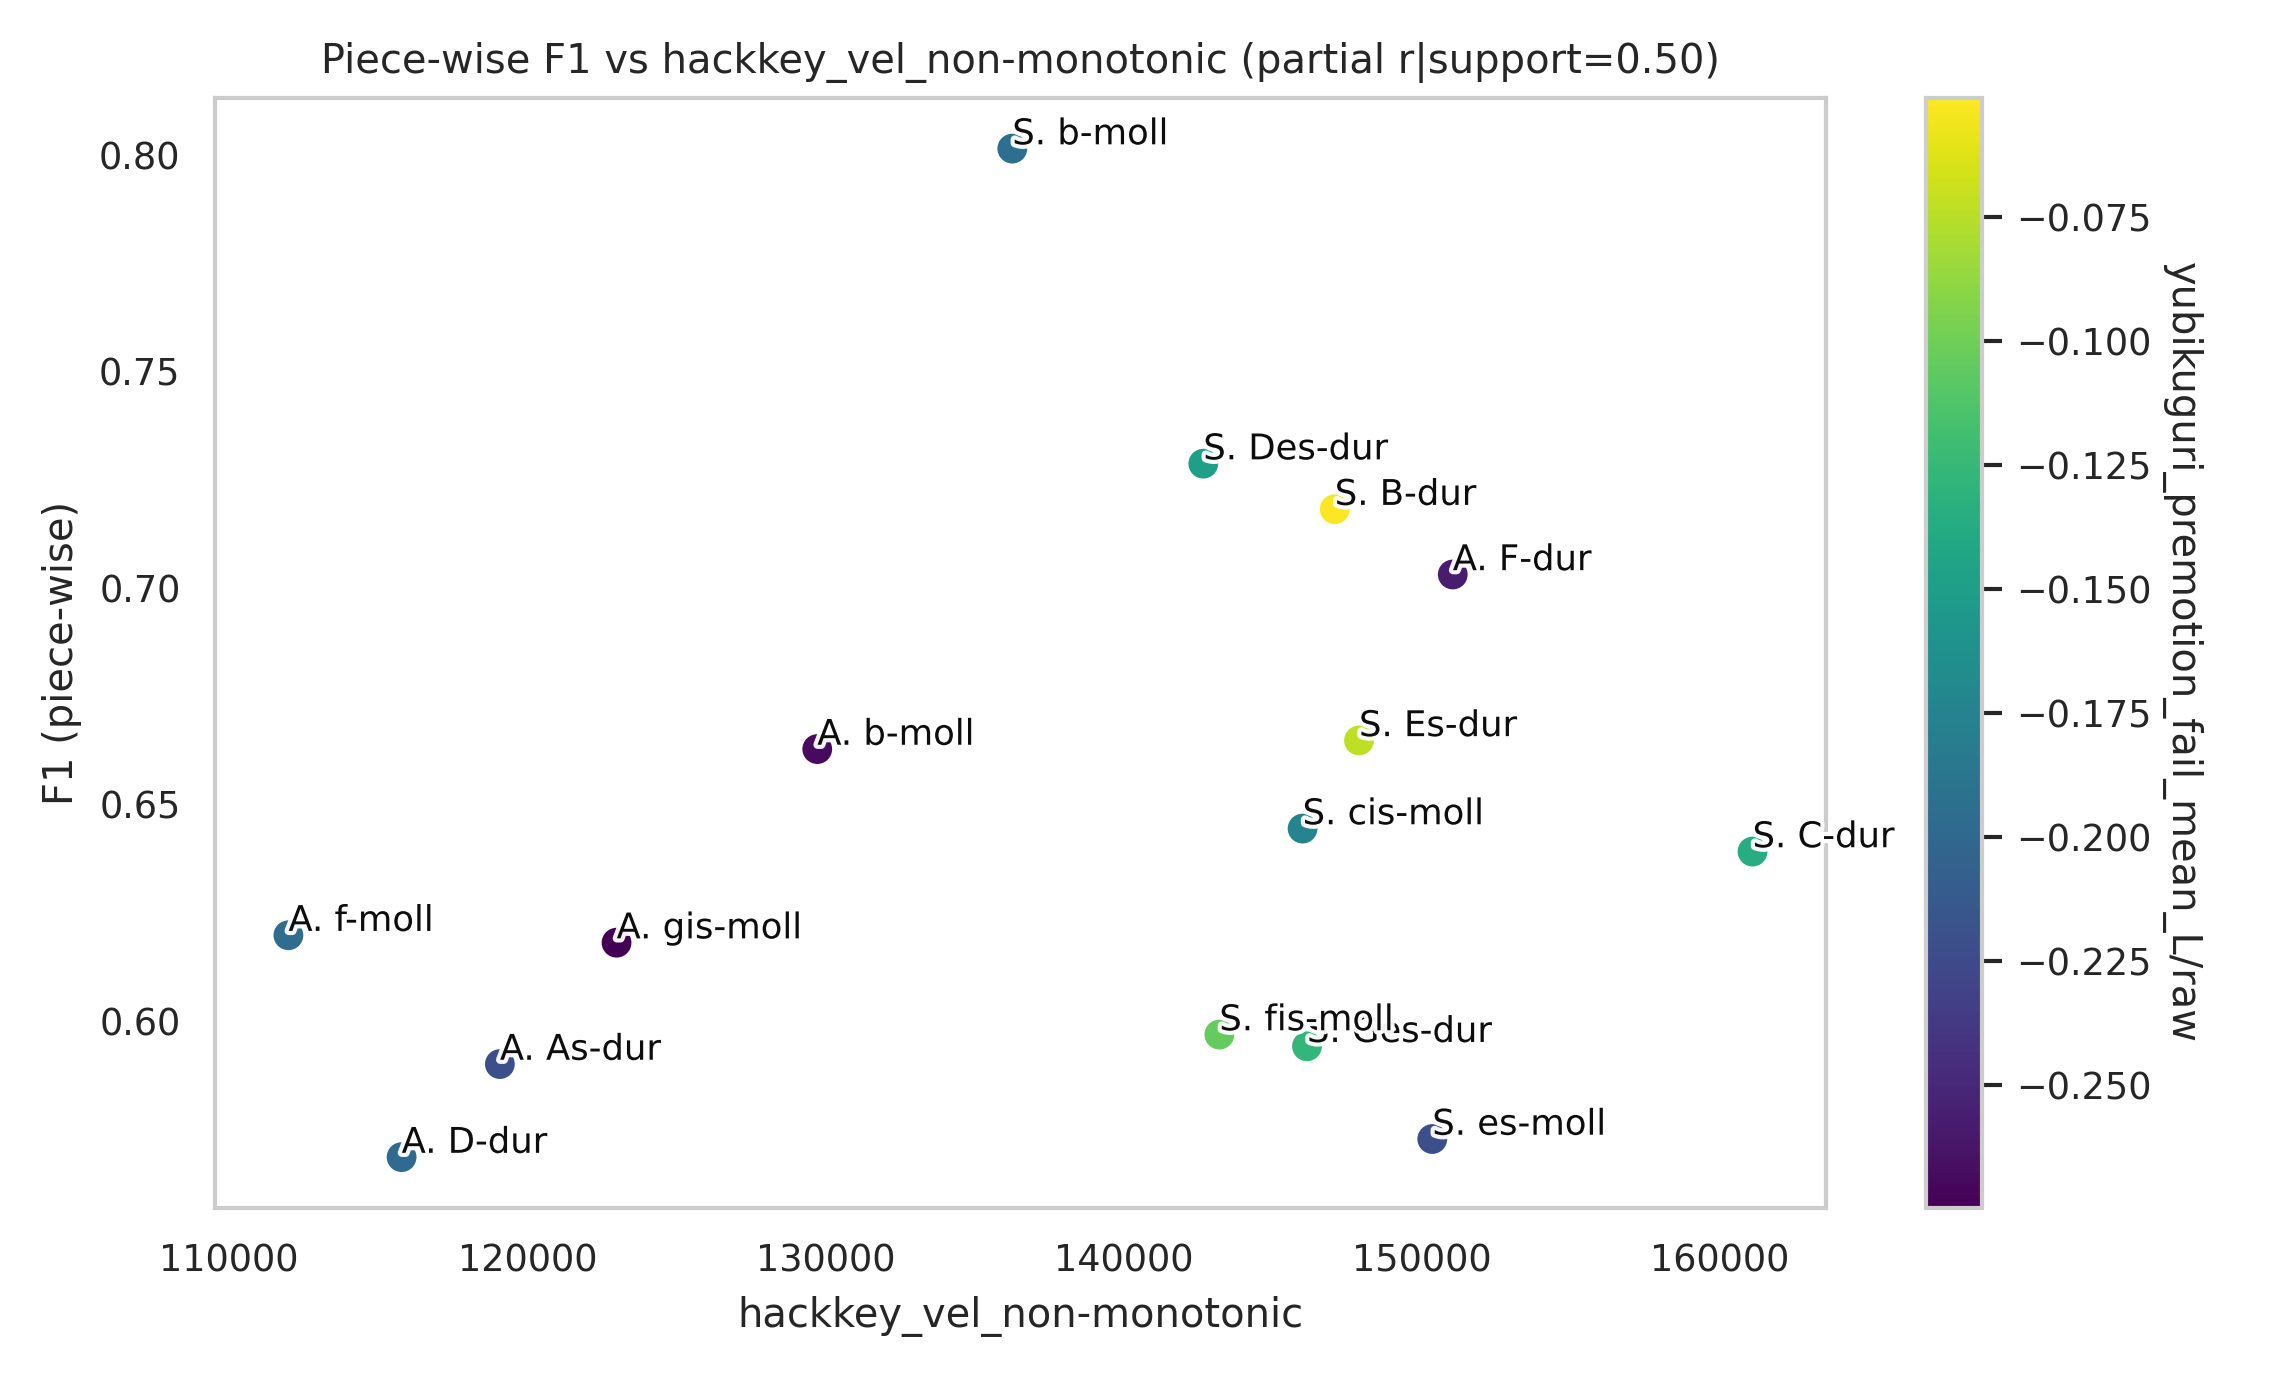
\includegraphics[width=0.95\linewidth]{figures/piece_f1_correlation.png}
  \caption{Piece-wise F1 versus the most positively correlated descriptor (colour indicates the second descriptor). Labels abbreviate pieces (S.=Scale, A.=Arpeggio).}
  \Description{Scatter of piece-wise F1 against top descriptor with colour as the second descriptor; points annotated with piece labels.}
  \label{fig:piece_f1_corr}
\end{figure}

\begin{figure}[t]
  \centering
  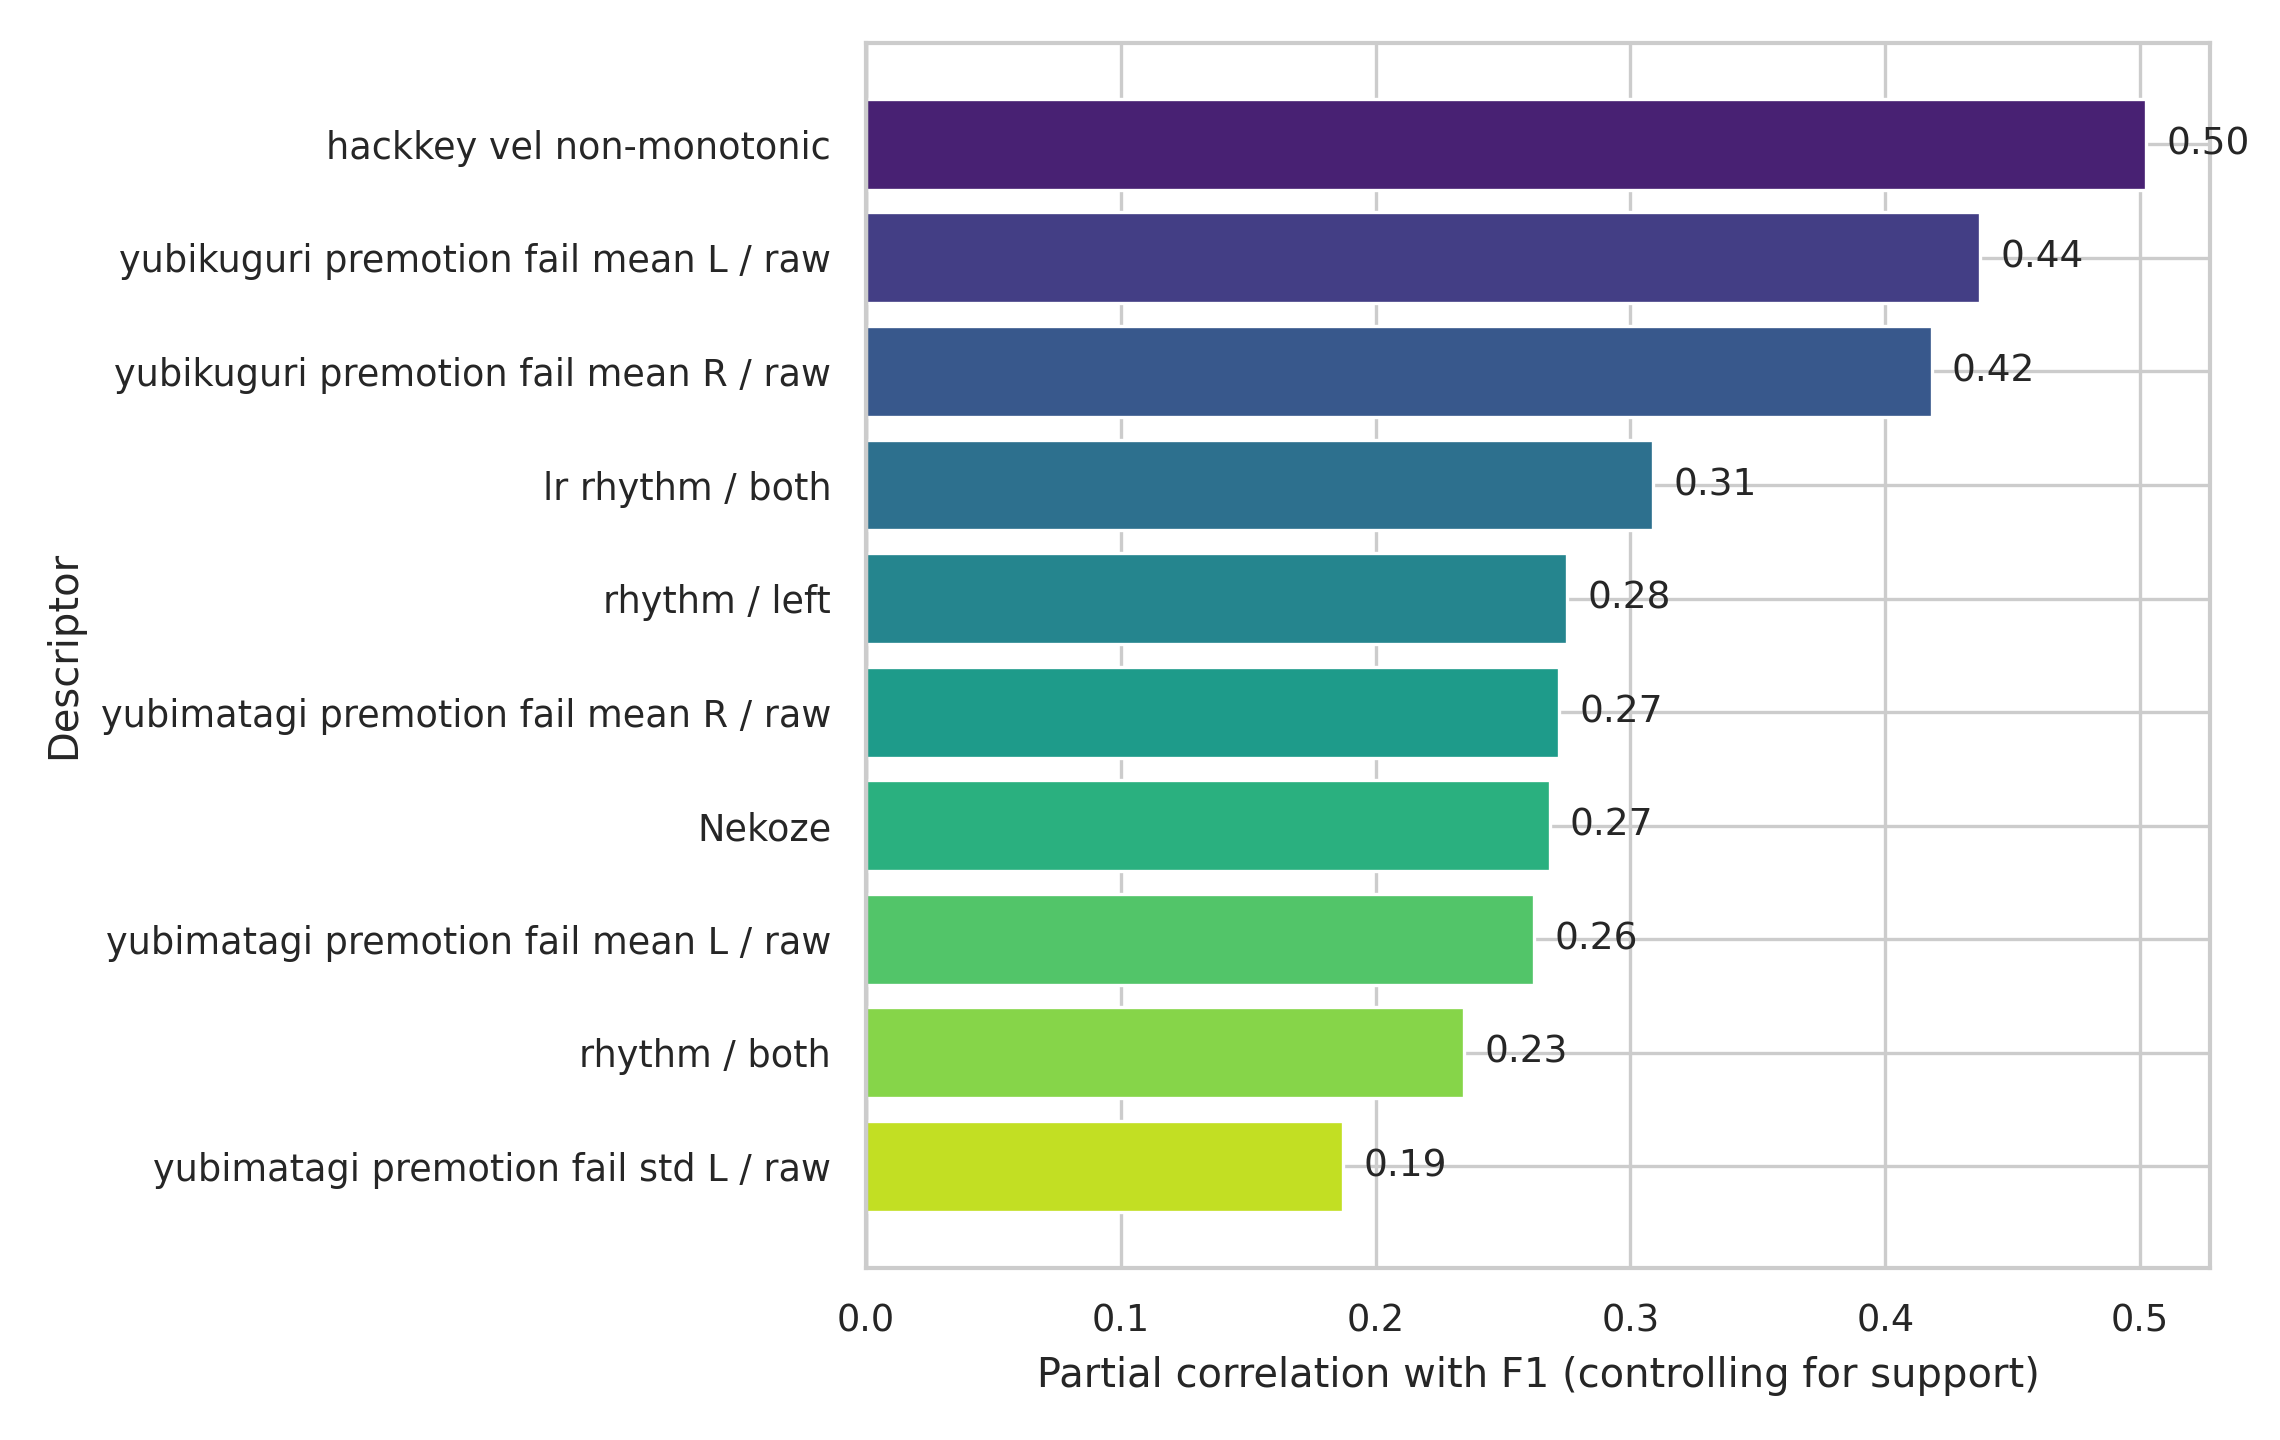
\includegraphics[width=0.95\linewidth]{figures/piece_f1_correlation_bar.png}
  \caption{Partial correlations (controlling for support) between piece-wise F1 and descriptors. Bars show the top descriptors excluding support-like variables; values annotated.}
  \Description{Horizontal bar chart listing descriptors on the y-axis and partial correlations with F1 on the x-axis, with numeric values on each bar.}
  \label{fig:piece_f1_corr_bar}
\end{figure}

\subsection{Highlight Validity (Amateur Weakness)}
% 日本語訳: ハイライトの妥当性(アマチュアの弱点の可視化)
We quantify whether severity hotspots focus \emph{where amateurs struggle} by measuring agreement with expert-marked spans on a curated Top‑20 set per annotator. For each recording we derive a frame‑level \emph{severity} from the model's time series (attention, evidence, or their product) and sweep light post‑processing (power $\gamma\in\{1.0,1.5,2.0\}$, smoothing window $w\in\{1,5,9\}$, global lag $\in\{-0.2,0.0,+0.2\}$~s). We report ROC‑AUC, AUPRC (AP), best F1/IoU across thresholds, and a point‑biserial correlation proxy.

\textbf{Agreement with individual annotators.} Averaged across eight annotators (320 rater–audio pairs), the \emph{audio} stream achieves ROC‑AUC $0.753$, AP $0.662$, best‑F1 $0.733$, best‑IoU $0.607$, and Pearson $0.385$. The \emph{sensor} stream is weaker but non‑trivial (ROC‑AUC $0.548$, AP $0.500$, best‑F1 $0.597$, best‑IoU $0.454$, Pearson $0.038$). In both cases, the \emph{attention} series with $w{=}9$ and a small lag performs best (audio: $+0.2$~s; sensor: $-0.2$~s), reflecting minor timing offsets.

\textbf{Consensus (group) ground truth.} Because coaching is subjective, we also aggregate annotators by frame‑wise vote proportion and threshold at $\geq0.5$ (minimum three annotators present). Against this consensus target, \emph{audio} agreement strengthens: ROC‑AUC $0.817$, AP $0.753$, best‑F1 $0.799$, best‑IoU $0.683$, Pearson $0.490$. \emph{Sensor} consensus metrics remain modest but usable (ROC‑AUC $0.529$, AP $0.517$, best‑F1 $0.625$, best‑IoU $0.475$). These results indicate that highlights concentrate on passages experts collectively deem coachable, supporting the paper's claim that localized highlights correspond to pedagogically salient spans.

\paragraph{Rater cohort.}
We recruited eight pianists to mark amateur-weak sections: three expert pianists (all with teaching experience), four conservatory students, and one student with conservatory-comparable piano skills. Since our focus here is not on comparing rater skill groups but on validating whether model highlights correspond to perceived weaknesses, we collectively refer to all raters as “pianists” unless an analysis explicitly distinguishes groups.

\paragraph{Annotation app and procedure.}
Raters used a local web application (Piano Performance Marker; see Figure~\ref{fig:annotation_ui}, source under \verb|/home/kazuki/Projects/Profy/piano-performance-marker|) to review predefined evaluation sets and mark weak sections by start/end time on a waveform. After login with a username, the app presents a fixed list of amateur recordings (Top‑20 set selected \emph{a priori} by the model’s amateur posterior under an SNR threshold and balanced across piece types); a size‑ and distribution‑matched random control set was also used. Raters can play/seek, adjust playback rate, and zoom; weak spans are added by dragging on the waveform, then edited or deleted in a sidebar list that shows per‑span duration and total time/percentage. A slider records an overall take‑level score. Keyboard shortcuts include Space (play/pause) and Enter (save+next); progress resumes from the last item on re‑login.

For each username/audio pair the app writes one JSON file with canonical fields: \verb|evaluation_id|, \verb|evaluator| (username), \verb|audio_filename|/\verb|audio_display| (name shown), \verb|audio_file| (compatibility alias), \verb|audio_index| (1‑based order), \verb|duration| (s), \verb|total_score| (0–10), and \verb|problem_sections| as a list of objects \verb|{start, end}| in seconds, plus \verb|evaluation_time| (epoch ms) and ISO \verb|timestamp|. Files are persisted under \verb|piano-performance-marker/evaluations/<username>/<base>.json| and synchronized into \verb|piano-performance-marker/web_evaluations| prior to analysis.

\begin{table}[t]
  \centering
  \caption{Top/bottom pieces by mean accuracy (multimodal; averaged over 3 folds). Values: mean accuracy and mean F1; $N$ indicates total support across folds.}
  \label{tab:piece_accuracy}
  \begin{tabular}{lccc}
    \hline
    Piece & Accuracy & F1 & $N$ \\
    \hline
    \multicolumn{4}{l}{Top 5} \\
    Scale b-moll & 0.819 & 0.801 & 437 \\
    Scale Des-dur & 0.791 & 0.729 & 440 \\
    Scale B-dur & 0.773 & 0.718 & 431 \\
    Arpeggio F-dur & 0.724 & 0.703 & 430 \\
    Scale cis-moll & 0.712 & 0.644 & 431 \\
    \hline
    \multicolumn{4}{l}{Bottom 5} \\
    Arpeggio f-moll & 0.646 & 0.620 & 431 \\
    Scale Ges-dur & 0.643 & 0.594 & 430 \\
    Arpeggio As-dur & 0.642 & 0.590 & 431 \\
    Arpeggio D-dur & 0.618 & 0.568 & 430 \\
    Scale es-moll & 0.599 & 0.573 & 427 \\
    \hline
  \end{tabular}
\end{table}

\begin{figure}[t]
  \centering
  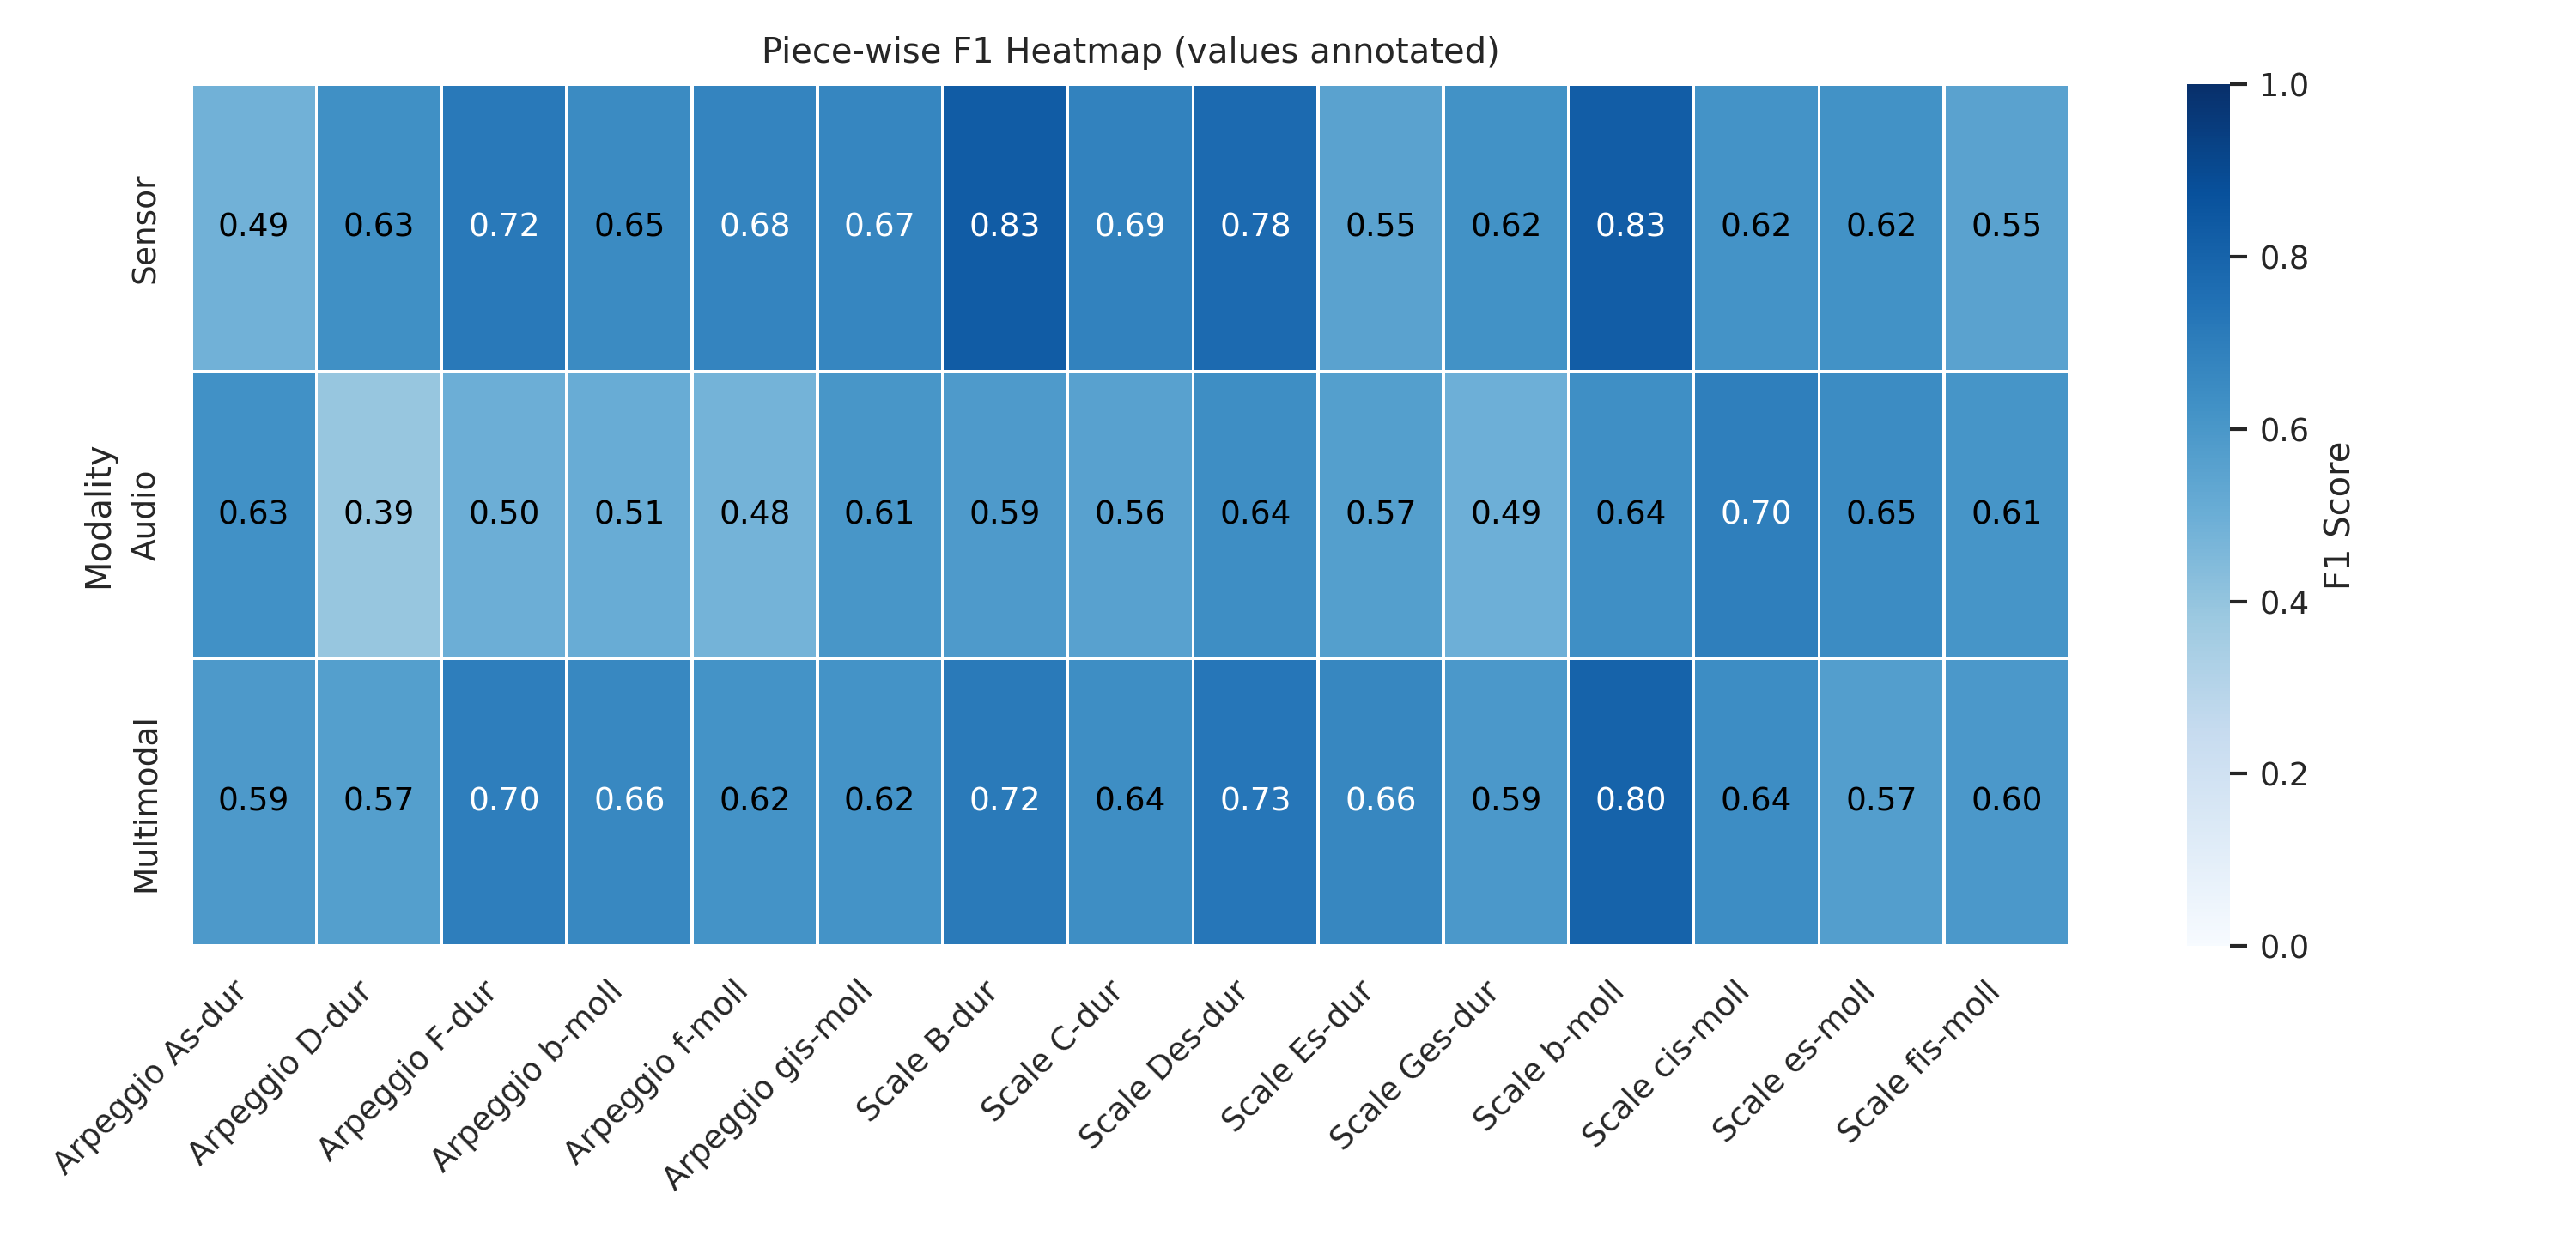
\includegraphics[width=1.0\linewidth]{figures/piece_f1_heatmap.png}
  \caption{Piece-level performance heatmap (averaged over 3 folds; values annotated).}
  \Description{Heatmap showing per-piece performance across folds.}
  \label{fig:piece_heatmap}
\end{figure}


\begin{figure}[t]
  \centering
  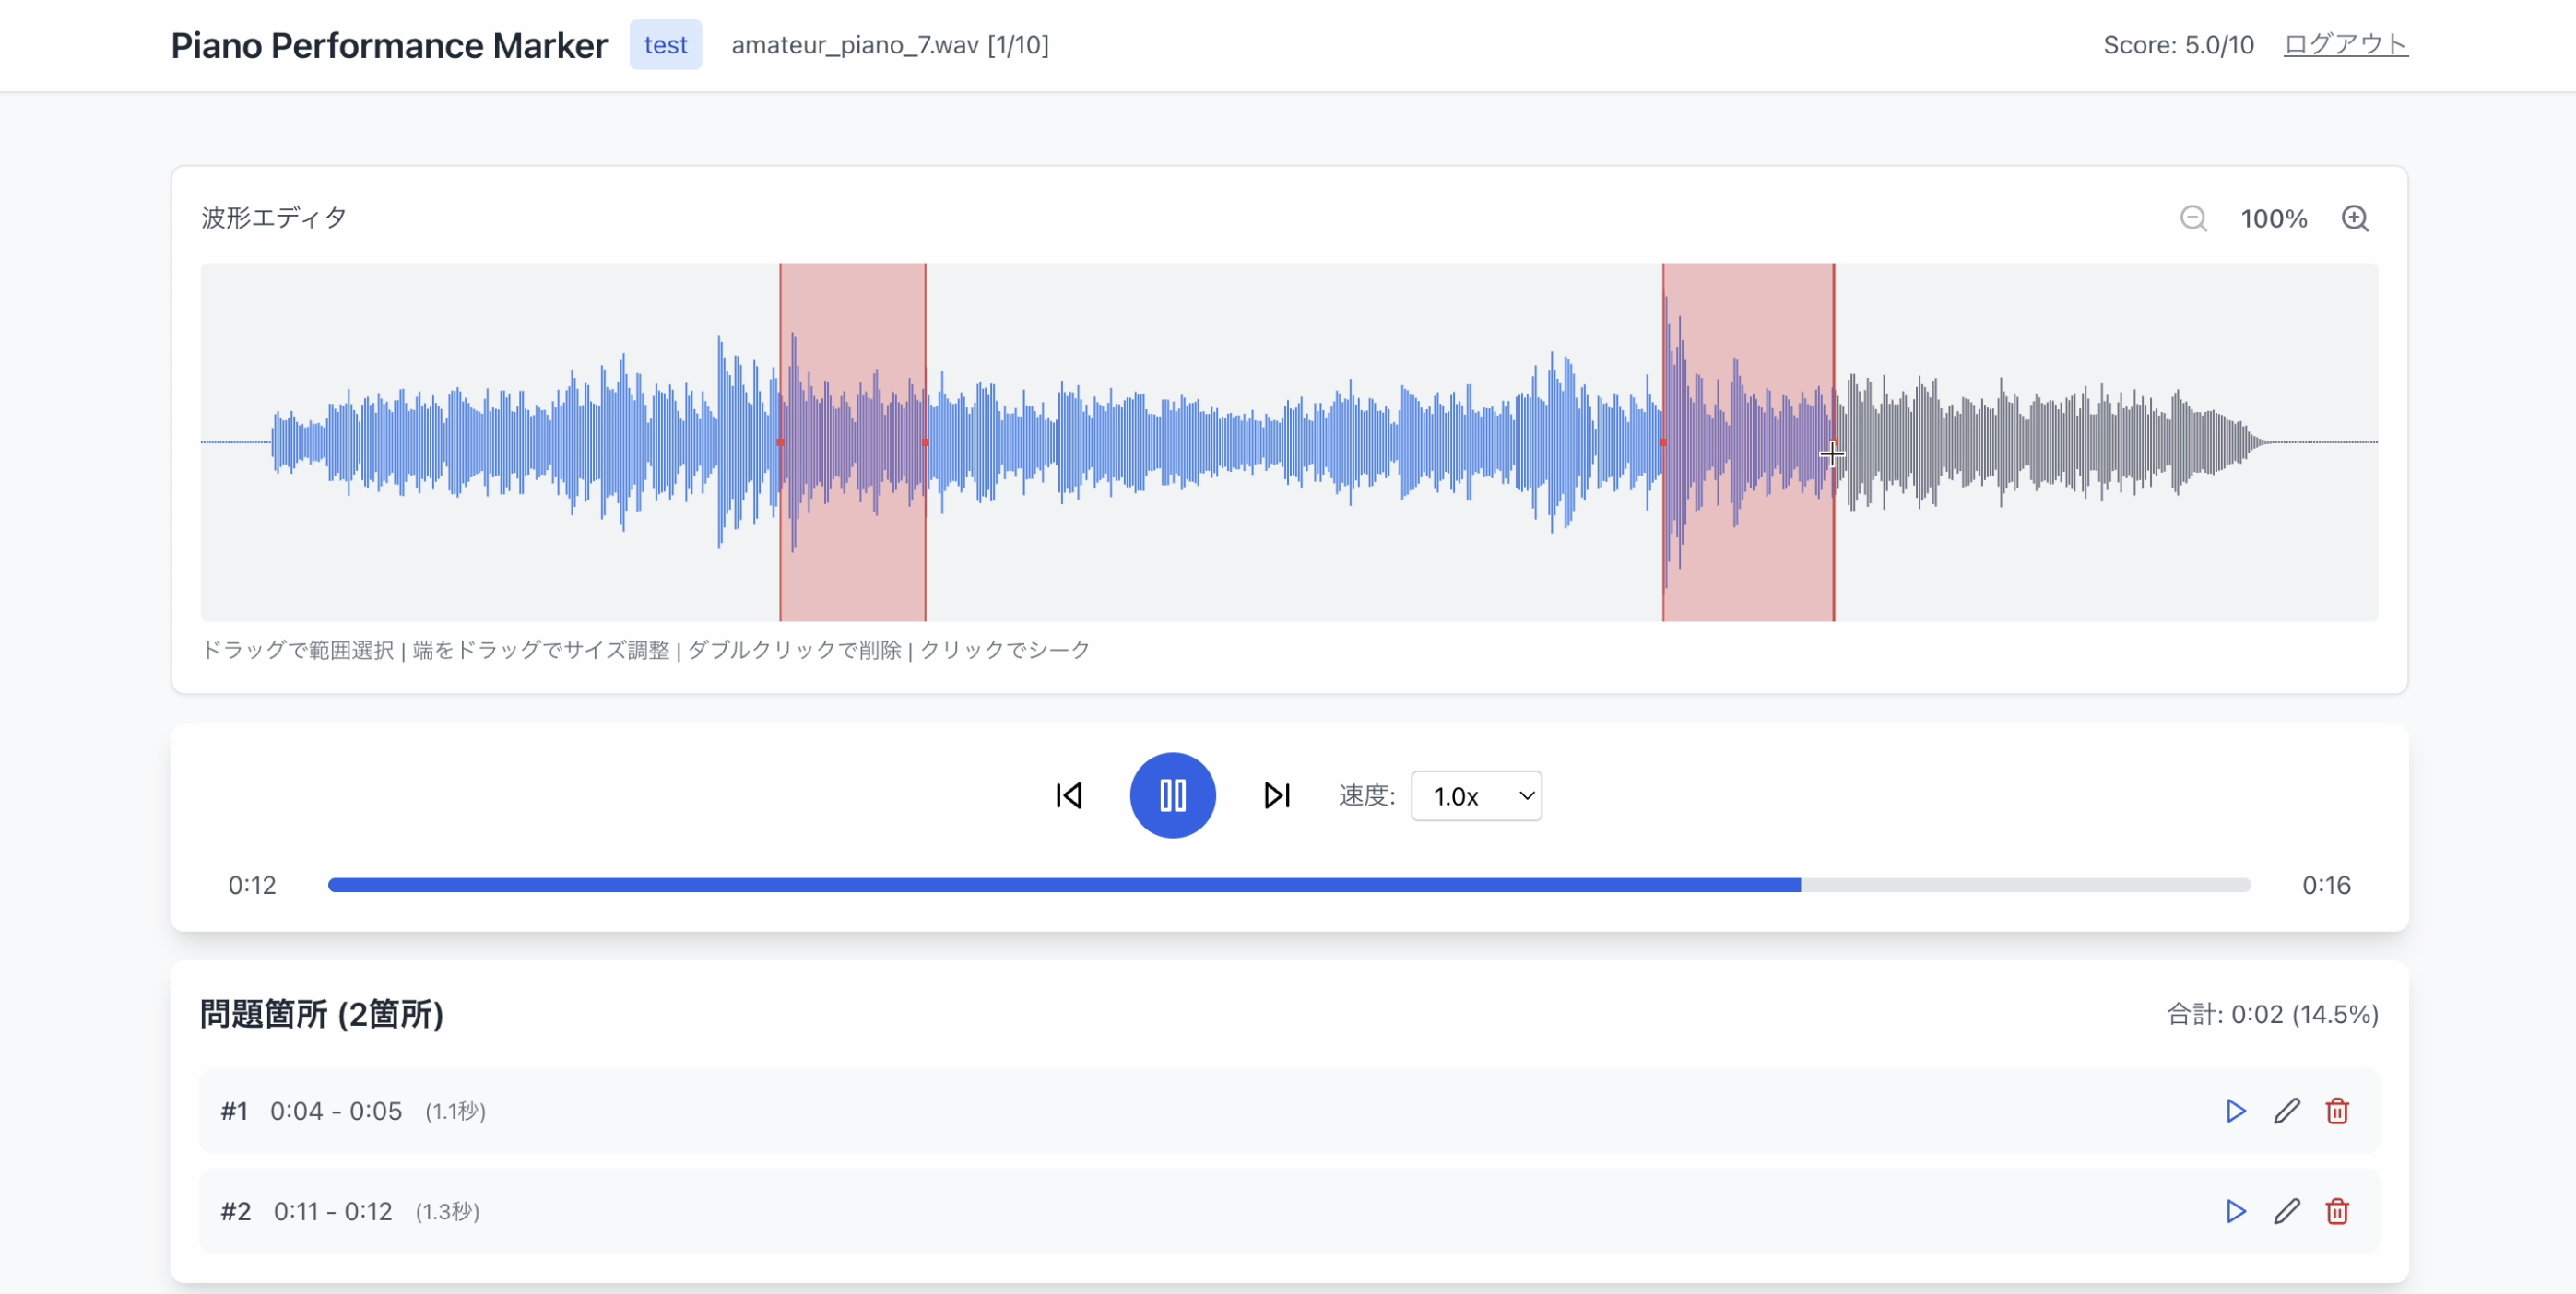
\includegraphics[width=0.95\linewidth]{figures/piano_marker.png}
  \caption{Expert annotation tool (Piano Performance Marker): raters listen and mark weak sections (start/end) on Top-20 amateur clips; JSON is persisted per rater/audio. We use these annotations to evaluate agreement between the model's highlighted spans and expert judgments.}
  \Description{Screenshot of the web UI used to collect expert attention/annotations, showing playback controls and segment selection.}
  \label{fig:annotation_ui}
\end{figure}

\subsection{Summary of Evaluation Results}
\begin{itemize}
\item \textbf{Performance snapshot}: Multimodal Macro-F1 $0.672\,\pm\,0.075$ (accuracy $0.698\,\pm\,0.043$); sensor-only $0.687\,\pm\,0.092$; audio-only $0.603\,\pm\,0.022$.
\item \textbf{Piece-wise analysis}: Piece-averaged accuracy $0.696$ with high accuracy on major/minor scales (e.g., Scale b-moll $0.819$) and lower accuracy on certain arpeggios (e.g., Arpeggio D-dur $0.618$).
\end{itemize}

% 日本語訳: これらの結果は、プロフィネットをプロのピアノのパフォーマンス評価のための実用的かつ効果的なシステムとして確立し、教育の設定や競争評価に適しています。
These results establish Profy as a practical and effective system for expert piano performance assessment, suitable for deployment in educational settings and competition evaluation.

\commentout{

% 日本語訳: 分析の視覚的説明は、注意深いパフォーマンスを強調することによって
\subsection{Visual Description of the Analysis by Highlighting Performance with Attention} \label{visualization_audio}
% 日本語訳: 上記の結果は、私たちの方法は、ピアノのパフォーマンスにおける一般的な音楽スキルよりも明るさの音楽表現をより正確に評価することができることを示していますので、私たちは明るさの表現の観点で視覚的なフィードバックに焦点を当てているので、音楽コーチングのための私たちの方法を適用することを目指しています音楽パフォーマンスを正確に分析する能力に基づいて。 私たちは、モデルの音楽表現を評価し、音楽実践者に有用なフィードバックを提供する能力を利用する方法を評価し、その結果、パフォーマンス分析モデルを音楽コーチングのための効果的なツールにします。
The result above shows that our method is able to more accurately assess the musical expression of the brightness than the general musical skill in piano performance.
Therefore, we focus on the visual feedback in terms of the brightness expression because we aim to apply our method for music coaching based on its ability to accurately analyze musical performances.
We evaluate how we can take advantage of the model's ability to assess the musical expression and 
provide useful feedback to music practitioners, thus making the performance analysis model an effective tool for music coaching.
% By visualizing the attention of the model, we can find which portions of the performances are deemed as more important than other portions for the performance analysis.

% 日本語訳: 図では、明るさの表現を変える上で非常に良いと考えられているプレイヤーのパフォーマンスに対する注意パターンを示しています。 図(a)は、明るくなる予定のパフォーマンスに対する注意を示し、専門家は実際にそれを明るく識別し、モデルはそうするが、図(b)は、暗くなる予定のパフォーマンスに対する注意を示し、専門家は実際にそれを暗く識別し、モデルはそうする。 これらの注意の視覚化を検証することによって、モデルはパフォーマンスの表現に応じて注意の異なるパターンを示すことがわかります。これは、注意のパターンの違いを視覚化することによって、明るさの表現を特定するためのパフォーマンスの重要な部分を特定することができることを示しています。 これらの注意地図を分析することで、モデルがスキル評価に重要だと考える要因についての洞察を得ることができます。
In Figure \ref{highlight_audio_0_hanon}, we show the attention patterns for the performances of a player who is deemed very good at altering the brightness expression.
Figure \ref{highlight_audio_0_hanon} (a) depicts the attention for the performance intended to be bright and the experts actually identify it as bright and so does the model, while Figure \ref{highlight_audio_0_hanon} (b) depicts the attention for the performance intended to be dark and the experts actually identify it as dark and so does the model.
By inspecting these visualization of the attention, we observe that the model shows the different patterns of the attention depending on the expression of the performance.
This suggests that we can identify the important portions of the performance for the identification of the brightness expression by visualizing the difference of the attention patterns.
By analyzing these attention maps, we can gain insight into the factors that the model considers important for the skill assessment.

\begin{figure}[t]
  \centering
  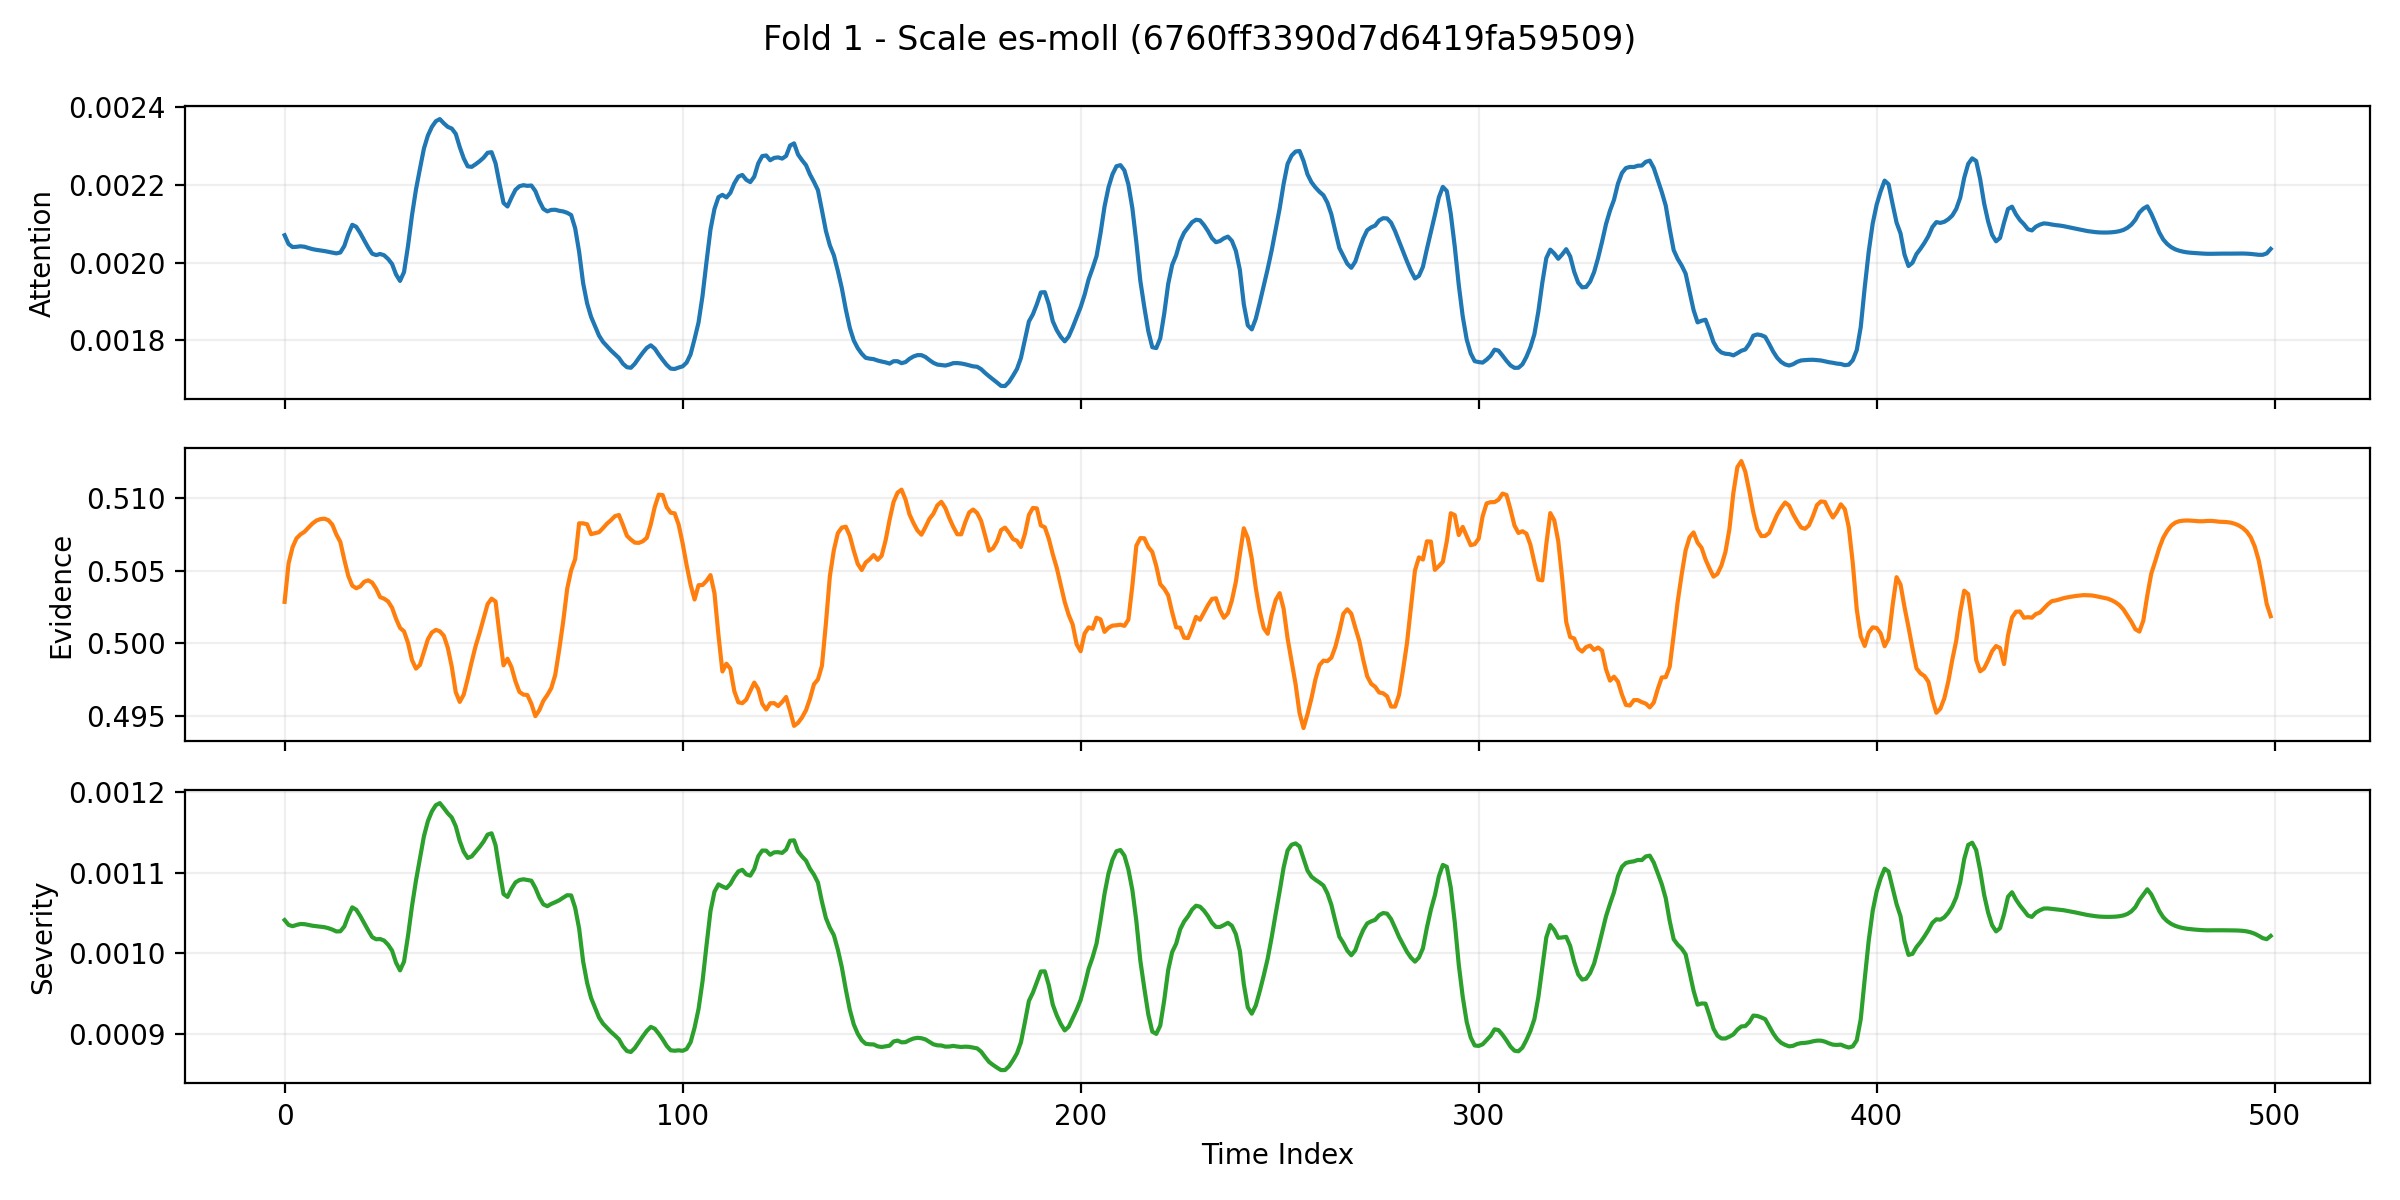
\includegraphics[width=\linewidth]{figures/highlight_audio_0_hanon.png}
% 日本語訳: パフォーマンスの表現はモデルの分析と一致します. (a) 明るい表現でパフォーマンスに注意を示し、 (b) 暗い表現でパフォーマンスに注意を示す。 注意は、パフォーマンスの表現に応じて異なるパターンを示しています。
  \caption{Time-series attention analysis for two renditions of Hanon exercise No.1. Severity highlights (red) reveal distinct focus regions when the performer targets bright versus dark tone, offering actionable guidance on articulation and voicing.}
% 日本語訳: ハノン練習曲の2つの演奏に対し、注意・証拠・重大度の時系列を表示し、明るい音色と暗い音色で異なる重視区間を可視化する。
  \Description{Three stacked line plots (attention, evidence, severity) for two versions of the same exercise, with shaded high-severity segments indicating passages emphasised by the model.}
  \label{highlight_audio_0_hanon}
\end{figure}

% 日本語訳: 別のプレイヤーでも、注意の視覚化から、意図した表現と評価の不一致を引き起こす箇所を同様に特定できる。
For other players as well, attention visualisation similarly exposes the passages that drive disagreement between intended expression and expert/model assessments, enabling targeted feedback without additional figures.

% 日本語訳: 注目パターンを参照として使用すると、どのパフォーマンスのパーツが反対評価の責任を負っているかを特定することができます。 このパターンは、パフォーマンスのこの部分がモデルが反対の評価を提供することを原因とし、プレイヤーが明るさの表現のスキルを向上させたいときに、その部分を深く調べることができることを示唆する可能性があります。
By using the attention pattern as a reference, we can identify which portions of the performance are responsible for the opposite assessment. 
For example, we find that the attention concentrates strongly approximately at the time from 1 to 1.5 seconds.
This pattern indicates that this portion of the performance would cause the model to provide the opposite assessment, possibly suggesting that the player can examine the portion in depth when they would like to improve their skill in brightness expression.

% 日本語訳: 私たちは、パフォーマンス分析モデルが異なる注意パターンを生み出し、その分析結果に基づいてパフォーマンスの重要な部分を強調する方法を示しましたが、私たちが認識しなければならないパフォーマンスのどのような要素を理解し、音楽スキルを向上させるために注意情報を活用する方法を理解することは簡単な課題ではありません。
We have demonstrated how the performance analysis model generates varying attention patterns and highlights important portions of a performance based on its analysis results. 
However, it is not a straightforward task to get insight into what kind of elements in the performance we have to discern and how to leverage the attention information to enhance the musical skills.

% 日本語訳: この時点で、最新の技術は、パフォーマンスオーディオファイルをMIDIフォーマットに転送することで、分析モデルは音楽スコアの視覚的なフィードバックを提供することを可能にし、ほとんどの音楽実践者が使用することを知っています。 このユーザーインターフェイスは、音楽スコアのビジュアルフィードバックが「AI分析」フィールドで分析結果を表示し、音楽ノートに関する強調情報を提供し、それらを赤に強調します。
At this point, the recent technology to transcribe performance audio files into the MIDI format \cite{hawthorne2021, gardner2022} allows the analysis model to provide visual feedback on musical scores, with which most music practitioners are familiar to use.
We show an example of an user interface for the visual feedback on musical scores in Figure \ref{UI}.
This user interface of visual feedback on musical scores shows the analysis result in the "AI Analysis" field and provides the highlight information over the musical notes by highlighting them in red.

% 日本語訳: ミュージカル・スコア・インターフェイスは、ミュージカル・スコア・インターフェイスがミュージカル・スコア・インターフェイスと調和しているため、ミュージカル・スコア・インターフェイスは、ミュージカル・スコア・インターフェイスと調和している。
The musical score interface allows music practitioners to playback and review their performances by targeting at the musical notes with highlight. That is because the performance recording within which the attention highlights is aligned to the musical score.
For instance, they are able to use the musical score interface in the following manner:
\begin{enumerate}
% 日本語訳: 1. 演奏後に「Highlight」ボタンを押してAI分析の結果を確認する。
   \item After their performance, check if they have performed in the correct way without anything wrong by clicking the "Highlight" button and obtaining the "AI Analysis" result.
% 日本語訳: 2. ハイライトされた音符を手がかりに問題箇所を特定する。
   \item If there is something wrong in the performance, they will find the spot where the things are going wrong based on the highlight on the notes.
% 日本語訳: 3. 問題箇所を確認したら緑のカーソルを移動して該当音符を選択する。
   \item Having identified where the things are wrong, they can move the cursor (colored in green in Figure \ref{fig:annotation_ui}) and select the note,
% 日本語訳: 4. 選択した音符から再生して重要な音響特徴を把握する。
   \item They playback and listen to the performance from the note they have selected and understand the important audio features.
% 日本語訳: 5. 理解した内容に基づき再演し改善を確認する。
   \item Based on the understanding, they perform again to see if they can improve their performance.
 \end{enumerate}
% 日本語訳: 上記のステップを通して繰り返しイターすることによって、音楽の実践者は徐々にエラーを示すエリアや改善のためのエリアを排除することができます。
By repeatedly iterating through the steps above, music practitioners can gradually eliminate highlighted areas indicating errors or areas for improvement. 
Once all such highlights have been addressed, they will have effectively mastered the skill.

% 日本語訳: 私たちは、音楽の明るさの表現に関して音楽スコアインターフェイス内での強調と再生のための同じ方法が他の音楽スキルに適用される可能性があることに留意します 私たちの方法は、モデルがスキルを十分な正確さで評価する限り、インターフェイスを通じて追加スキルに関する視覚的なフィードバックを提供することができます。 たとえば、モデルの一般的な音楽スキルの評価の正確さが、明るさの表現の評価の正確さと比較できるならば、それは音楽スキルの信頼性の高い参照と見なすことができます。
We note that the same method for highlight and playback within the musical score interface regarding musical brightness expression can be applied to other musical skills. 
Our method can offer visual feedback regarding additional skills through the interface, as long as the model assesses the skill with sufficient accuracy. 
For instance, if the model's accuracy in assessing general musical skills is comparable to its accuracy in assessing brightness expression, we can consider it a reliable reference for the musical skill.
It is then reasonable to derive highlights from its attention, and provide similar visual feedback on musical scores.
}

% ======================================================================
% Section: Discussion
% ======================================================================
\section{Discussion}

\subsection{What the technical evaluation establishes}
Our study set out to test three claims: that weak supervision can still yield localized signals useful for practice, that multimodal fusion can be made robust rather than brittle, and that interpretability can be preserved without sacrificing headline accuracy. The results in \S\ref{sec:technical-eval} support all three. Although the model is trained only with performance-level labels, the multiple-instance objective, together with sparsity and temporal-smoothness regularization, consistently concentrates evidence on a small number of decisive instants. Those high-evidence moments appear where teachers routinely intervene—near phrase boundaries, finger crossings, and marked dynamic changes—and the qualitative agreement we observe with expert markings indicates that the inductive biases we built in are aligned with pedagogy rather than merely producing plausible overlays. At the same time, we deliberately separated the optimization pathway that drives the numeric decision from the pathway that produces UI-facing evidence. Decision-level fusion is used for robustness, while mid-level attention and evidence remain stable for explanation; this separation prevented accuracy tuning from eroding the readability of the highlights.

\subsection{Why some pieces separate expertise better than others}
Piece-wise analysis clarifies the structure behind the global scores. Major and minor scales tend to yield higher separability than arpeggios. Scales demand long stretches of strict bimanual synchrony and economical thumb-under transitions; amateurs accumulate micro-delays and velocity dips at crossings, while experts keep inter-hand drift and variance low. These sub-100\,ms phenomena are recorded faithfully by the key sensors and therefore become reliable cues. By contrast, arpeggios require wider hand relocations and piece-specific compensations, especially in keys with many accidentals, which blur class boundaries and reduce the consistency of cues across takes. This pattern suggests a principled repertoire for diagnosis or placement: a small set of scales spanning contrasting key signatures, complemented by one or two arpeggios with controlled leaps, can maximize separability while covering distinct motor demands. Formally, repertoire selection can be posed as choosing items that increase mutual information between piece identity and the expertise label while maintaining coverage of evenness, crossings, span, and relocation.

\subsection{What sensors know that audio forgets, and when fusion helps}
The modality results are consistent with intuition about the sensing channels. High-rate key-motion signals carry motor-control variables that the acoustic channel tends to smear: pre-touch latency, key travel profiles, aftertouch, and release asymmetries. Pedal use, soundboard resonance, and room response mask or smooth these micro-events in the waveform. Sensors therefore dominate on passages where evenness and economy at crossings differentiate skill. Audio becomes valuable when the discriminative signal lives in voicing and balance among parts, or when articulation choices alter spectral envelopes in ways not fully predictable from key motion. In such cases, cross-modal attention lets the audio stream resolve ambiguities in the sensor stream and improves classification. Fusion does not uniformly exceed the best single stream because it is conditioned by reliability. When acoustic SNR is low, alignment is imperfect after time normalization, or model capacity is constrained, the quality-aware gate is right to favor sensors and the combined score may match rather than exceed the sensor baseline. Conversely, for pieces where voicing is structurally salient, multimodal models outperform either stream alone by pooling complementary information.

\subsection{From localized evidence to amateur-facing interaction}
Although this paper focuses on visualizing expertise differences rather than deploying a tutor, the results already constrain the design of an effective amateur-facing interface. A productive loop is discover–focus–refine. Immediately after a take, the system should present overlays whose opacity reflects severity and whose labels use teacher-native vocabulary such as left–right rhythm drift, uneven crossings, or voicing imbalance. Focusing then narrows attention to a highlighted span with one-click looping, metronome anchoring, hand-solo playback, and call–and–response between the learner’s recording and a chosen reference exemplar at a matched tempo. Refinement closes the loop by re-recording and re-highlighting, showing deltas rather than absolute values so that improvement is perceptible and motivating. Uncertainty should be surfaced in situ by suppressing overlays when acoustic quality indicators are poor, maintaining appropriate trust calibration. A speculative UI sketch embodying this loop is shown in \Fig~\ref{fig:future_ui}.

\begin{figure}[t]
  \centering
  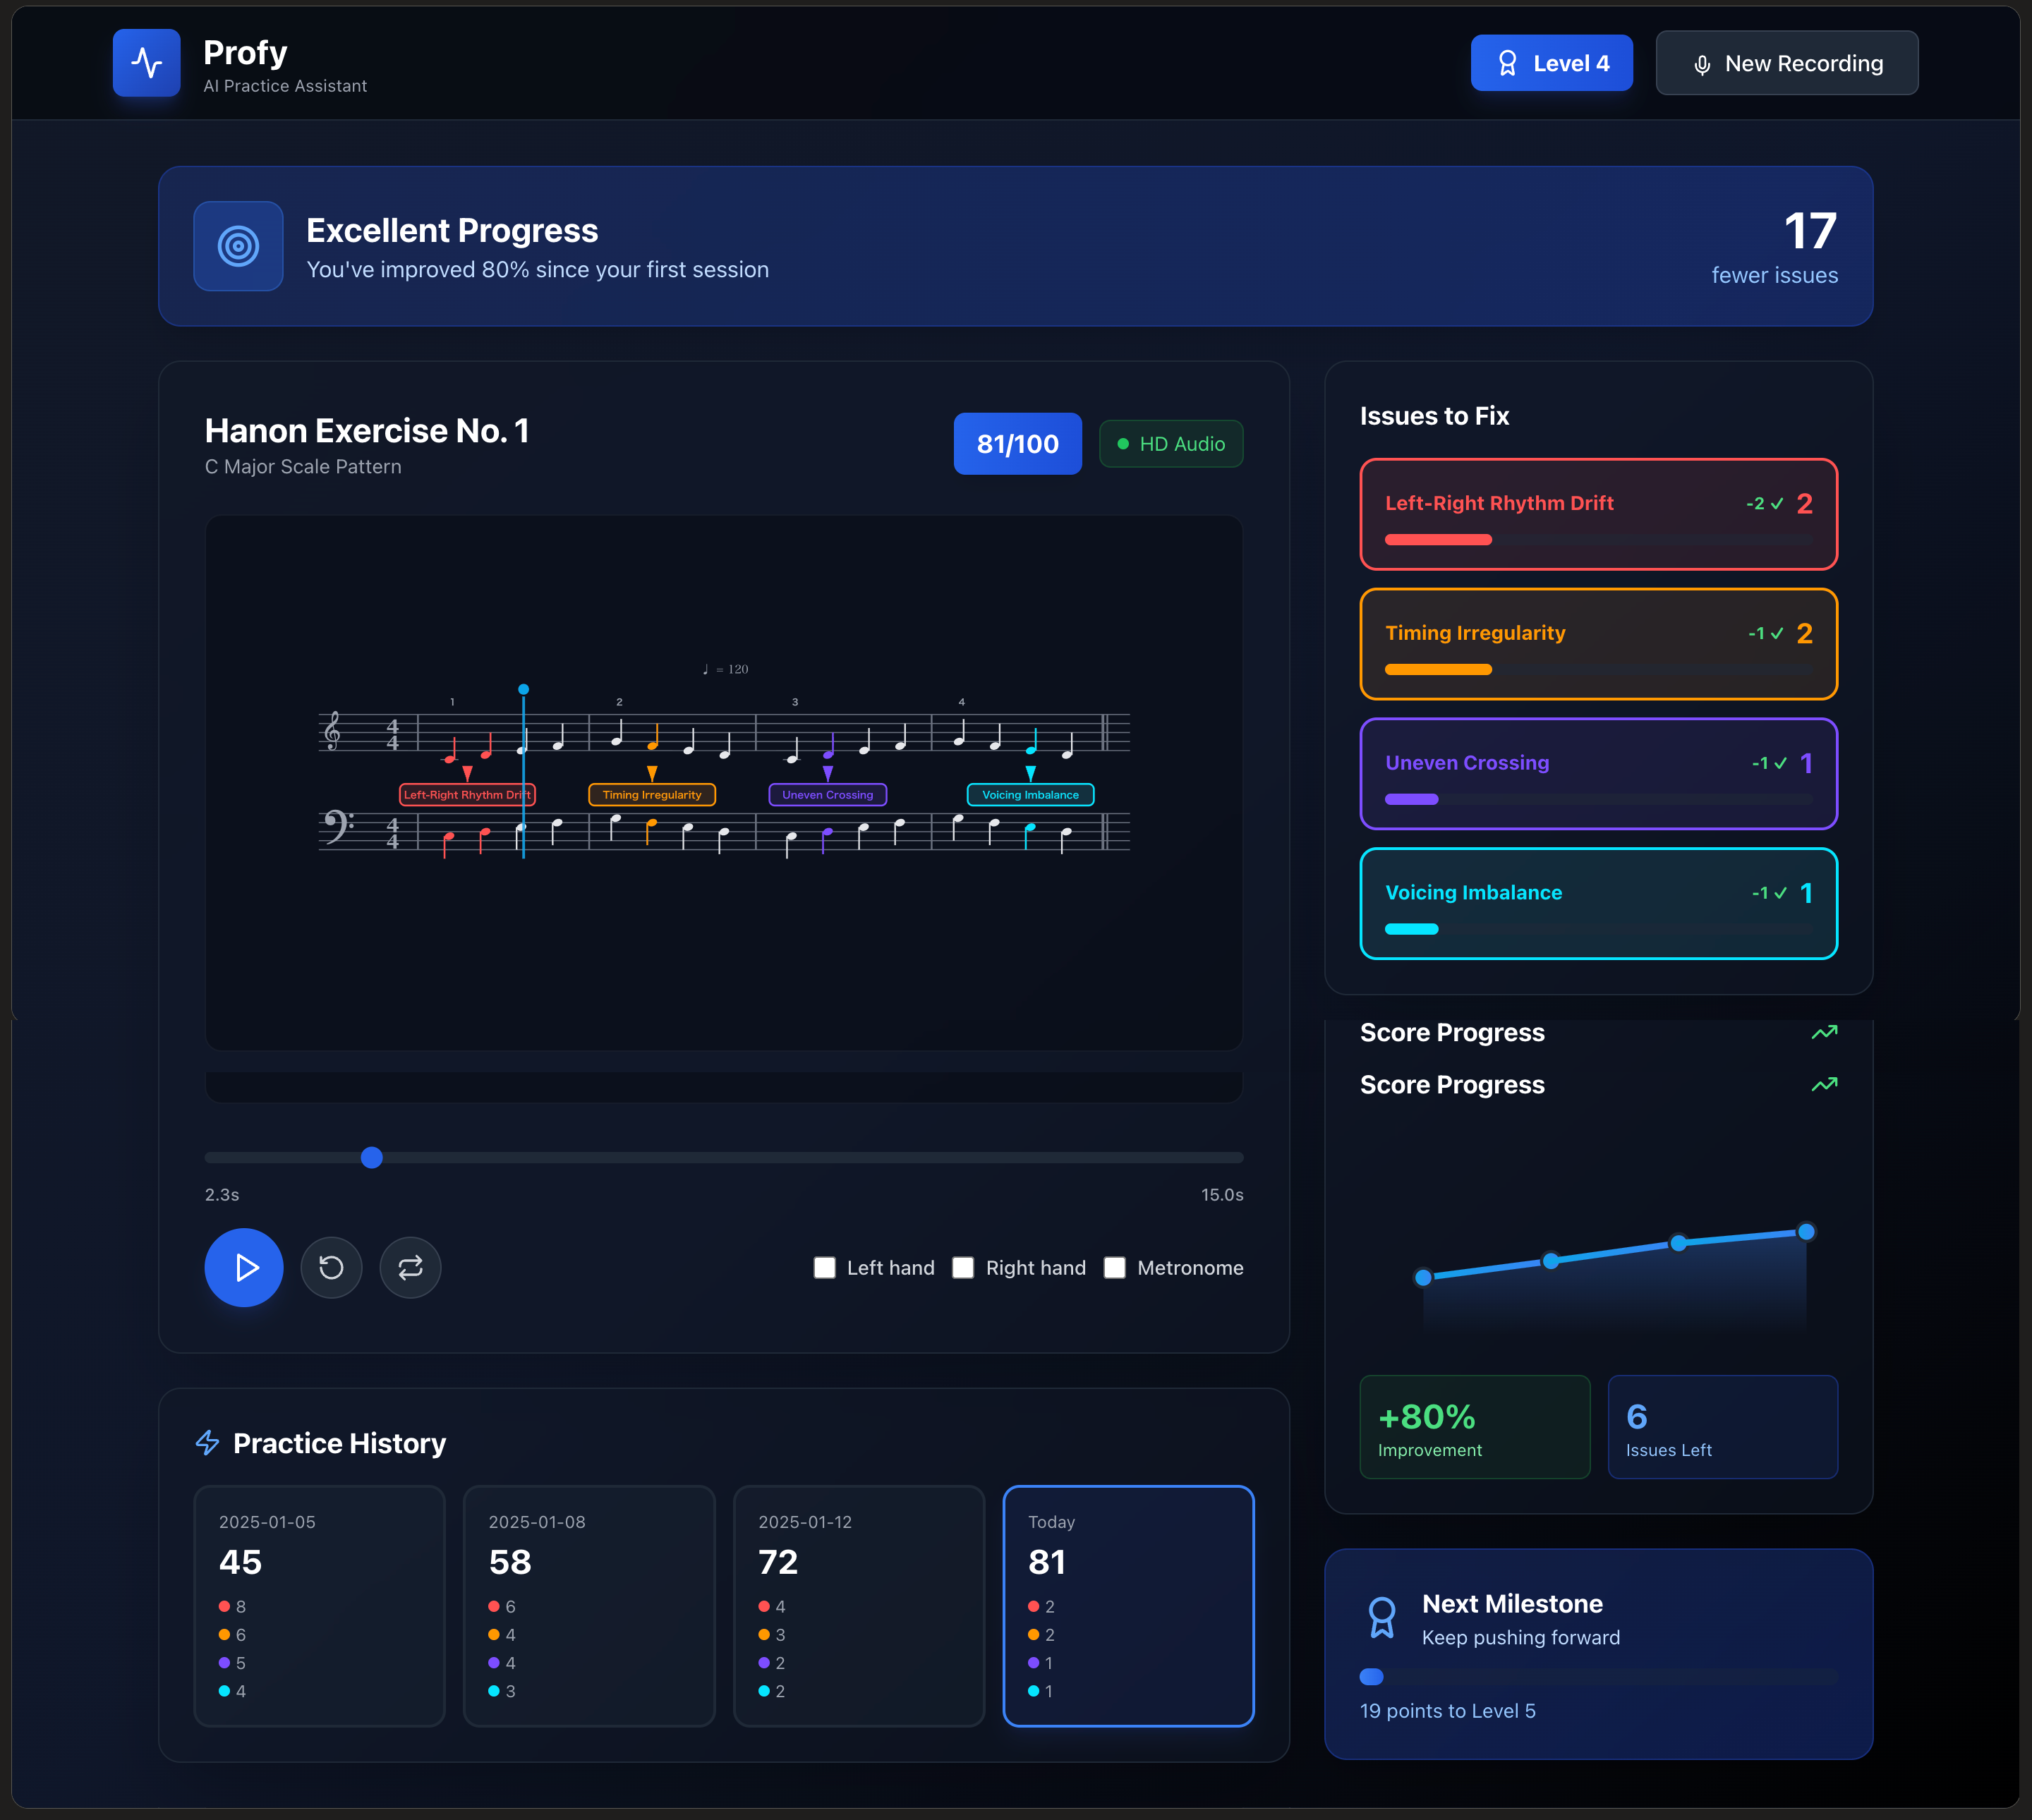
\includegraphics[width=0.98\linewidth]{figures/future_ui.png}
  \caption{Speculative amateur-facing UI embodying the discover–focus–refine loop. After a take, severity-weighted overlays highlight likely issues (e.g., left–right rhythm drift, uneven crossings, voicing imbalance). Focusing tools provide one-click looping, metronome anchoring, hand-solo playback, and call–and–response with a selected expert exemplar at a matched tempo. Refinement re-records and re-highlights, emphasizing deltas to make improvement perceptible; reliability indicators suppress overlays when input quality is poor.}
  \Description{Composite mockup showing score-aligned red overlays on a musical staff and timeline; controls for loop in/out, metronome on/off, left/right-hand solo, and call-and-response playback with an expert recording; a severity slider and reliability flag that disables overlays when quality is low.}
  \label{fig:future_ui}
\end{figure}

\subsection{Mimesis as a design principle rather than an obstacle}
A mimesis-first view of creative learning provides a principled frame for these interactions. From classical accounts to contemporary cognitive perspectives, the ability to recognize and reproduce another performer’s stylistic signature appears to be a precondition for meaningful personal deviation. Profy’s localized highlights make those signatures audible and visible at the granularity of beats and note groups. The interface should therefore encourage intentional imitation before exploration by allowing learners to select among multiple expert exemplars—including a teacher’s own recording—and by exposing similarity measures between the learner’s take and each target along dimensions that the model already localizes, such as crossing regularity or inter-hand synchrony. Once imitation is secure on a span, the same controls can scaffold controlled departures, making individuality a consequence of competence rather than a substitute for it.

% (Removed future work subsection by request.)

% ======================================================================
% Section: Conclusion
% ======================================================================
\section{Conclusion}

This paper introduced Profy, a weakly supervised and interpretable system that localizes where amateur and expert piano performances differ and renders those differences directly on the score. Despite training on performance-level labels only, the model produces time-indexed evidence that concentrates at musically meaningful micro-structures and qualitatively aligns with expert markings. Across pieces, high-rate key-motion sensors carry most of the separability signal by preserving motor-control regularities that audio often blurs, while audio contributes in passages where voicing and balance matter; fusion helps in those cases but need not dominate when reliability is uneven. The contribution is therefore a lens rather than a tutor: an analysis pipeline that turns coarse labels into score-synchronized highlights suitable for guiding attention during practice. In short, expertise differences are not only measurable; they are renderable in situ, creating common ground for learners and teachers.


% \begin{acks}
acknowledgements
In Figure 1, the icons are made by Freepik from www.flaticon.com.
\end{acks}

%%
%% The acknowledgments section is defined using the "acks" environment
%% (and NOT an unnumbered section). This ensures the proper
%% identification of the section in the article metadata, and the
%% consistent spelling of the heading.
% \begin{acks}
% acknowledgements
% This work was partially supported by JST Moonshot R\&D Grant Number JPMJMS2012, JST CREST Grant Number JPMJCR17A3, and The University of Tokyo Human Augmentation Research Initiative.
% \end{acks}

%%
%% The next two lines define the bibliography style to be used, and
%% the bibliography file.
% 日本語訳: ACM リファレンス フォーマット リファレンス/リファレンス、リファレンス/リファレンス_1_初心者、リファレンス/リファレンス_2_中間、リファレンス/リファレンス_3_中間、リファレンス/リファレンス_4_スピーチ
\bibliographystyle{ACM-Reference-Format}
\bibliography{references/references}

\end{document}
% 日本語訳: エンドインポート
\endinput
%%
%% End of file `sample-authordraft.tex'.
